\chapter{System Maintenance}

\section{Environment}

\subsection{Software}

\begin {itemize}
	\item Python 3
	\item IDLE
	\item PyQt
	\item SQLite 3
	\item SQLite Database Browser
	
\end {itemize}

\subsection{Usage Explanation}


The table below includes all the listed software from the previous section with the explanation as to why I used them.
The listed software can be downloaded for free which made the creation of my system an easier approach. Also, this would mean that my client wouldn't need to purchase anything.

\begin{center}
\begin{tabular}{|p{4cm}|p{8.5cm}|}
\hline
\textbf{Software} & \textbf{Usage Explanation} \\ \hline

Python 3 & I used Python because it was the only programming language I was familiar with as I learnt how to use it during my time at sixth form. \\ \hline
IDLE & I used IDLE to write the Python scripts and since I am the most familiar with this software , it made implementation of the client application easier. \\ \hline
PyQt& PyQt included everything needed to create the graphical user interfance for my system and there was a lot of information on PyQt accessible which helped me create the graphical interface more effectively. \\ \hline
SQLite3 & Although this came with python, I have used this to create the database and manipulate the database as it was  easy for me to understand on how to do so and was very effective in doing so. \\ \hline
SQLite Inspector & This software helped me make the system's code relating the database a much more easier process because it allowed me to observe whether the database queries excutely correctly or not. \\ \hline

\end{tabular}
\end{center}
\subsection{Features Used}

\begin{center}
\begin{tabular}{|p{4cm}|p{8.5cm}|}
\hline
\textbf{Software} & \textbf{Features Used} \\ \hline

Python 3 & I took advantage of the ability to import modules to structure my code clearer.  \\ \hline
IDLE & There are countless number of features that IDLE has to offer which helped me create the application but I will mention a few of them. The syntax highlighter made it easier to understand the code that I was writing which is important when a system is complex(helps track what you are doing). Also it prevented me from making more errors. For example, I was able to spot out straight away if i mispelt a keywork such as print or while, etc. The 'Go to File/Line' feature when an error occurs, helped me tremendously as it was the main factor of helping me debug my program. Being able to run the system allowed me to test the system \\ \hline
PyQt& PyQt has many features that allowed me to create graphical user interface (GUI) for my system. The core components that I used to create the GUI were main windows, dialog boxes and widgets. \\ \hline
SQLite3 &I was able to create the database for the system through SQLite3. I used most of core features that was available to me through SQLite3 such as being able to ADD, DELETE,UPDATE to/from the database. Enforcing referential integrity was useful as it helped the database to become consistent.   \\ \hline
SQLite Inspector& I mainly used 'Browse Data' to check whether I have added, deleted or updated a record successfully. I also used 'Execute SQL' for the SELECT statements in the apllication as it allowed me to see whether the SQL query was correct or not.  \\ \hline

\end{tabular}
\end{center}

\section{System Overview}

%use as many subsections as necessary for the system components
\subsection{System Component}

\subsubsection{Graphical User Interface (GUI)}
Having a graphical user interface for the system makes it a lot more userable, giving the user a much more user friendly experience. Including a GUI makes it easier for the user to navigate around the system. I have used a QMainWindow and a QDialog to create the graphical user interface.

\subsubsection{Manage Item Menu}
The item menu can be managed at any time through the menu bar 'Item Menu'. The user can add/delete/update an item. \\

To add an item to the menu, the user must select 'Add Item'. By selecting 'Add Item', the user will be presented with a layout that consists of a table widget displaying all the records of the item menu and the fields (QLineEdits) which will be used to input information for the new item. \\

Deleting an item off the menu can also be found under the 'Item Menu' menu by selecting 'Delete Item'. The user will be presented with a layout that contains the same table widget that displays all records of the menu and has either the choice to delete an item by inputting the item name or the item ID. \\

The user also has the option to update an item's price. To do this, the user must select 'Update Item Price' where the user will be presented with a layout that contains the same the item menu table widget as the add and delete item layout. The user would have to input the ID of the item and the new price then click on the 'Update Item' button to update an item's price.


\subsubsection{Manage Bookings}

The user will be able to add/delete and update bookings. To do this, the user could either selection these options through "Bookings" on the menu bar or click on the 'Manage Bookings' button at the bottom of the main screen. \\

Clicking on the button will switch the central widget to the manage bookings widget where the user will be presented with the Bookings table widget where all of the booking records will be displayed and below the widget are the QPushButtons "Add Booking" and "Delete Booking". Clicking on Add Booking will then present the user with the same table widget and the required fields which the user would have to successfully fill to add a booking. As for the "Delete Booking"  QPushButton, the user will be presented with the same Bookings table widget and an input field for the user to input the selected booking they would like to delete and a "Delete BookingID" QPushButton to proceed the deletion. \\

The "Bookings" menu bar also has 3 options; "Add Bookings", "Delete Booking" and "Update Booking". The add/delete booking options are the same as described in the paragraph above. As for the "Update Booking" option, the user will be presented with the usual Bookings table widget and the input fields to update the booking.  

\subsubsection{Manage Sit-In Orders}

To manage an order, the user must select the table radio button and click on the "Select Table" QPushButton. If the table is unoccupied then the user would have to assign a customer to the table ( A QDialog box will pop up telling the user to assign a customer to the selected table). After assigning a customer to the table, the table will be known as 'occupied' which would allow the user to select that table without assigning a customer to that table everytime. So now that the table is occupied, there will be a manage order QDialog box where the booking details will be displayed using QLabels on a row at the top of the box. The dishes and drinks ordered will be split into two table widgets, the dishes ordered will be displayed on the left and the drinks on the right. \\

The user has all the neccessary options on the manage order box such as "Add", "Delete", "Finish", "Invoice Preview" and "Print Invoice" QPushButtons. The "Add" QPushButoon would be used to add items to the order, the "Delete" QPushButton will be used to delete items off the order, the "Invoice Preview" will show the user what the invoice would look like for the order, the "Print Invoice" will print the invoice and the "Finish" button will set the status of the table as unoccupied, clearing the booking details for that table and so the user would have to assign a customer to that table when selecting the table from the main screen.


\section{Code Structure}

%use as many subsections as necessary for the code sections
%the code below can be uncommented and used to get a code section from a particular file

\subsection{Displaying a table}
\begin{figure}[H]
    \pythonfile[firstline=36,lastline=51]{./Implementation/GUI/table_display.py}
\end{figure}

Above are the show\_results and show\_table functions which is part of the table\_display.py module. I needed to display tables on many widgets and so I created a module based around the show\_results and show\_table so that I all had to do was import this module and call the functions whenever I needed to display a table.

\subsection{Switching central widgets}
\begin{figure}[H]
    \pythonfile[firstline=494,lastline=504]{./Implementation/GUI/main_window.py}
\end{figure}
The functions shown above are used to switch the central widgets. I have created this in such a way so that I could just call the function whenever there was a click connection. Also, this was helpful because since there is a menu bar, the menu bar is used as an alternative to switch the central widget and so I could just call the connect functions above. 
\section{Variable Listing}

\begin{center}
\begin{longtable}{|p{3cm}|p{4.5cm}|p{3cm}|p{1cm}|}
\hline
\textbf{Variable Name} & \textbf{Purpose} & \textbf{Line numbers} & \textbf{Section} \\ \hline
%add booking .py
regExp & Holds the regular expression to only allow the user to enter letters for name inputs & 31 & 4.10.1\\ \hline
regexp & Holds the regular expression to only allow the user to input digits & 42 &4.10.1 \\ \hline
regexp2 & Holds the regular expression to only allow the user to input digits & 48 &4.10.1 \\ \hline
each & Stepper variable used in the for loop &57, 58 &4.10.1 \\ \hline
self.maximumdate&Used to set maximum date for QDateEdit &63 &4.10.1 \\ \hline
self.minimumdate&Used to set minimum date for QDateEdit &64 &4.10.1 \\ \hline
FirstName&Used to store user input &106, 119 ,121 &4.10.1 \\ \hline
LastName & Used to store user input & 107, 119, 121 &4.10.1 \\ \hline
TeleNumber&Used to store user input  &108, 119, 121 & 4.10.1\\ \hline
NumberOfPeople&Used to store user input &110, 119, 135 & 4.10.1\\ \hline
TableNumber&Holds the index of the table number combo box &113, 129, 135 &4.10.1 \\ \hline
BookingDate & Used to store user input & 114, 135 & 4.10.1\\ \hline
BookingTime&Used to store user input &115, 135 & 4.10.1\\ \hline
customer&Holds the variables FirstName,LastName and TeleNumber to create a record for Customers &121 & 4.10.1\\ \hline
db&Stores the path of the database &123,129,137 & 4.10.1\\ \hline
booking& Holds the variables customerid, TableNumber, NumberOfPeople, BookingDate and BookingTime to create a record for Bookings& 135 &4.10.1 \\ \hline
%add item to menu.py
regexpp& Holds the regular expression to only allow a maximum of 20 letters & 35 &4.10.2 \\ \hline
ItemName & Used to store user input & 72 &4.10.2 \\ \hline
ItemPrice & Used to store user input & 73 &4.10.2 \\ \hline
ItemType & Holds the selected index of the item type combo box & 73,74,76,78,79 &4.10.2 \\ \hline
MenuItem & Holds the variables ItemName, ItemPrice and ItemType to create a record for Items & 79 &4.10.2 \\ \hline
%add item to order.py
self.bookingDetails & Holds booking details such as bookingid, customerid, booking date, booking time, table number and number of people & 16&4.10.3 \\ \hline
bookingID & Holds booking id & 57 &4.10.3 \\ \hline
self.ItemID & Used to store user input & 58 &4.10.3 \\ \hline
Quantity & Used to store user input & 59 & 4.10.3\\ \hline
addedAlready & Holds a boolean value to indicate whether an item has been added to the order already (Used to increase quantity) & 61, 66, 83, 97, 128, 130 &4.10.3 \\ \hline
newQuantity & Used to calculate the new quantity after adding/deleting an item that's already been added to an order & 72 & 4.10.3\\ \hline
updateOrder & Holds the new quantity and item id to update the record & 73 &4.10.3 \\ \hline
itemsOrdered & Holds an array of ordered items for a particular booking & 98, 111&4.10.3 \\ \hline
%assign table customer
css & Holds the cascade style sheet code for the application&19 &4.10.4 \\ \hline
Date & Holds the system date & 120 &4.10.4 \\ \hline
Time & Holds the system time & 121 &4.10.4 \\ \hline
self.CustomerList & Holds an array of customer id's that has a booking on a certain table and date & 152, 166, 176 &4.10.4 \\ \hline
CustomerLastName & Holds an array of last names from the customer ids in self.CustomerList & 167, 184, 188 &4.10.4 \\ \hline
%delete item off order
OneQuantity & Holds a boolean value to indicate whether the quantity of an ordered item is one or not &82, 84, 112, 124, 117 & 4.10.8\\ \hline
%main window.py
self.TableOne Occupied & Holds a boolean value to indicate whether table one is occupied or not &34, 227 &4.10.9 \\ \hline
 self.TableTwo Occupied &Holds a boolean value to indicate whether table two is occupied or not &35, 241 & 4.10.9\\ \hline
self.TableThree Occupied &Holds a boolean value to indicate whether table three is occupied or not &36, 255 &4.10.9 \\ \hline
 self.TableFour Occupied&Holds a boolean value to indicate whether table four is occupied or not &37, 269  & 4.10.9\\ \hline
     self.TableFive Occupied &Holds a boolean value to indicate whether table five is occupied or not &38, 283 &4.10.9 \\ \hline
     self.TableSix Occupied &Holds a boolean value to indicate whether table six is occupied or not &39, 297 &4.10.9 \\ \hline
     self.TableSeven Occupied & Holds a boolean value to indicate whether table seven is occupied or not&40, 312  & 4.10.9\\ \hline
     self.TableEight Occupied&Holds a boolean value to indicate whether table eight is occupied or not & 41, 326 &4.10.9 \\ \hline
     self.TableNine Occupied &Holds a boolean value to indicate whether table nine is occupied or not &42, 340  &4.10.9 \\ \hline
     self.TableTen Occupied &Holds a boolean value to indicate whether table ten is occupied or not & 43, 354 &4.10.9 \\ \hline
     self.TableEleven Occupied&Holds a boolean value to indicate whether table eleven is occupied or not &44, 368  &4.10.9 \\ \hline
     self.TableTwelve Occupied &Holds a boolean value to indicate whether table twelve is occupied or not &45, 382  & 4.10.9\\ \hline
     self.TableThirteen Occupied &Holds a boolean value to indicate whether table thirteen is occupied or not &46, 396 &4.10.9 \\ \hline
     self.TableFourteen Occupied& Holds a boolean value to indicate whether table fourteen is occupied or not&47, 410 &4.10.9 \\ \hline
     self.TableFifteen Occupied &Holds a boolean value to indicate whether table fifteen is occupied or not &48, 424 &4.10.9 \\ \hline
     self.TableSixteen Occupied &Holds a boolean value to indicate whether table sixteen is occupied or not &49, 438 &4.10.9 \\ \hline
tableList & Used to store the number of tables for the radio button widget & 154,156 &4.10.9 \\ \hline
Todays Date & Holds the system date & 171 &4.10.9  \\ \hline
%manage order
self.Finished & Holds a boolean value to indicate whether the table/booking has finished &24, 188 & 4.10.11 \\ \hline
self.TotalPrice & Used to store the total price of all ordered items& 149, 181 &4.10.11 \\ \hline
self.price & Holds an array of all the prices of all ordered items&150, 160, 162 &4.10.11 \\ \hline
self.quantity & Holds an array of quantities of all ordered items & 151, 173, 174, 175 & 4.10.11\\ \hline



\end{longtable}
\end{center}

\section{System Evidence}

\subsection{User Interface}

\begin{landscape}

\begin{figure}[H]
    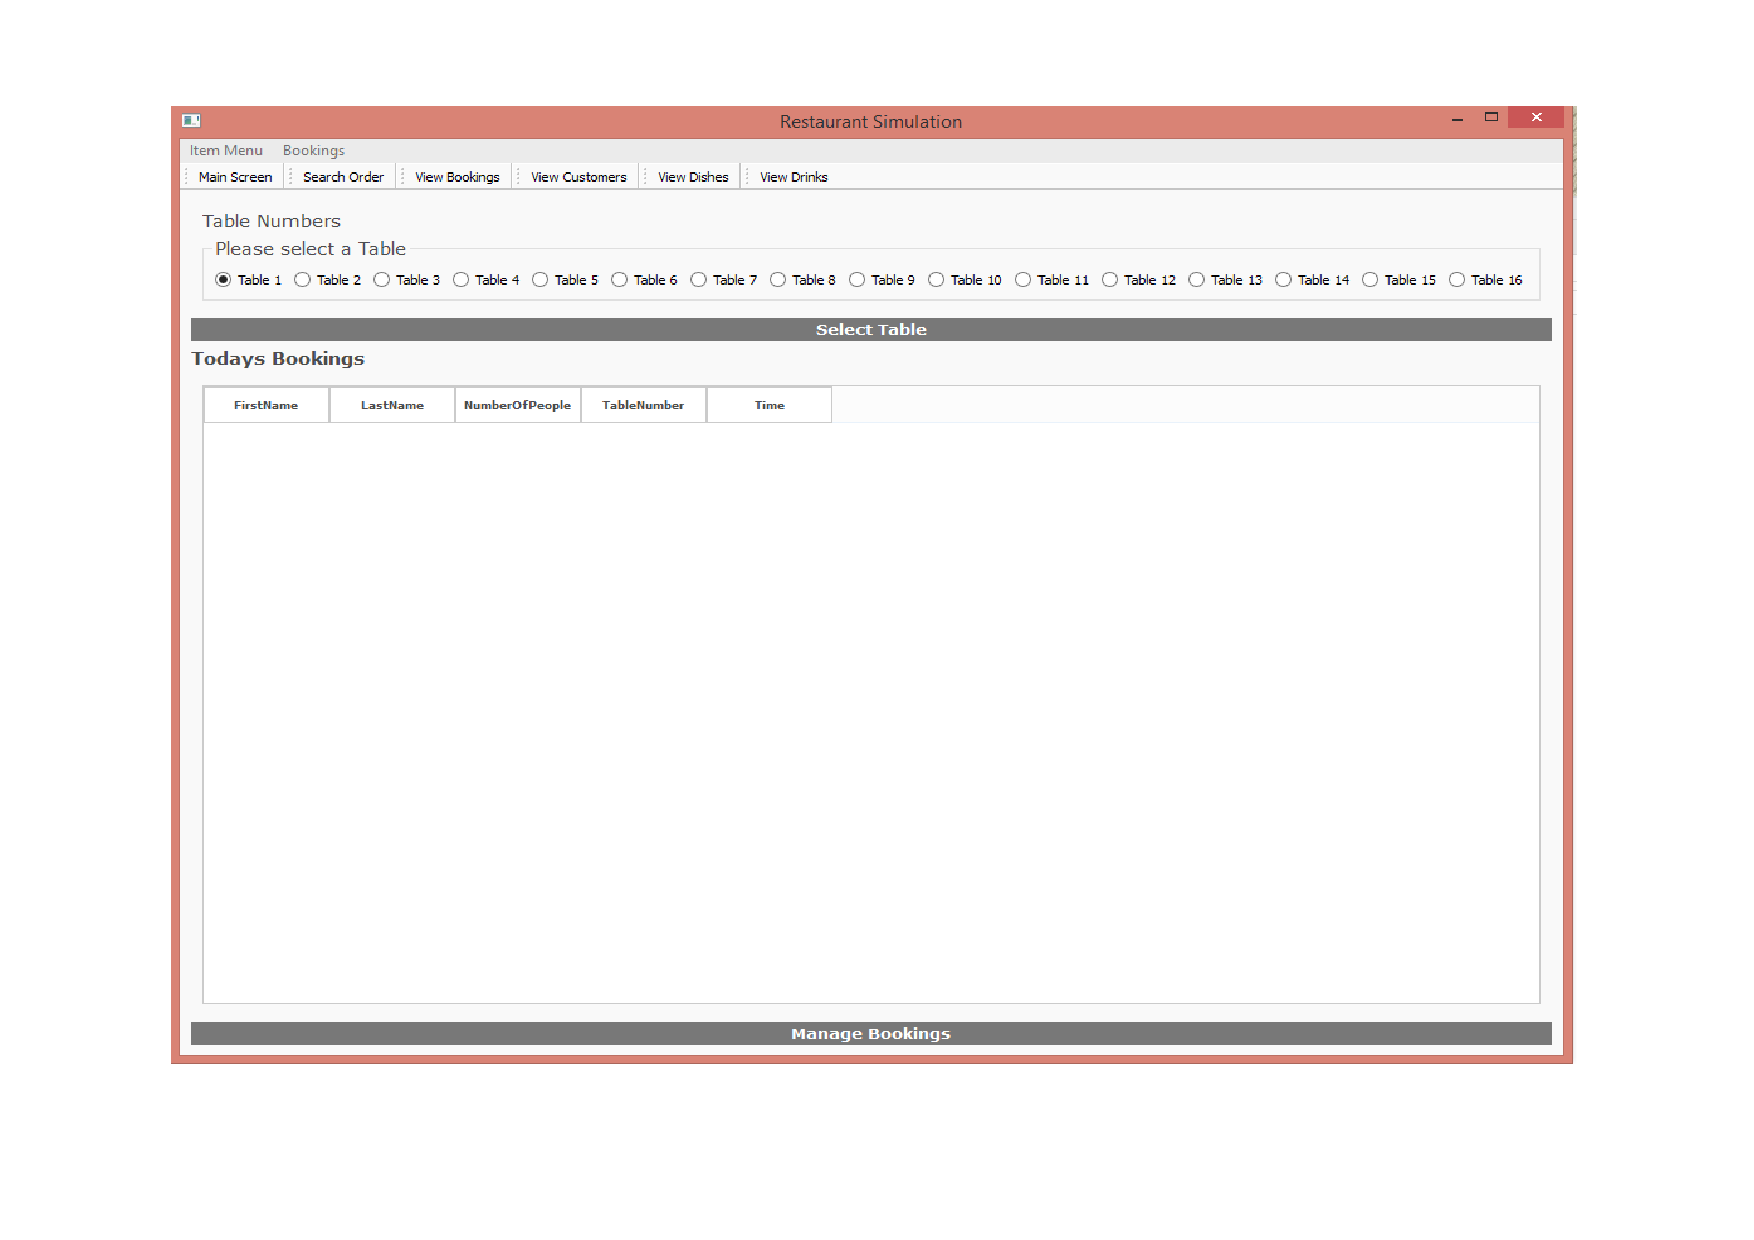
\includegraphics[height = 15cm]{./Maintenance/images/screen1}
    \caption{} \label{fig:screen1}
\end{figure}

\begin{figure}[H]
    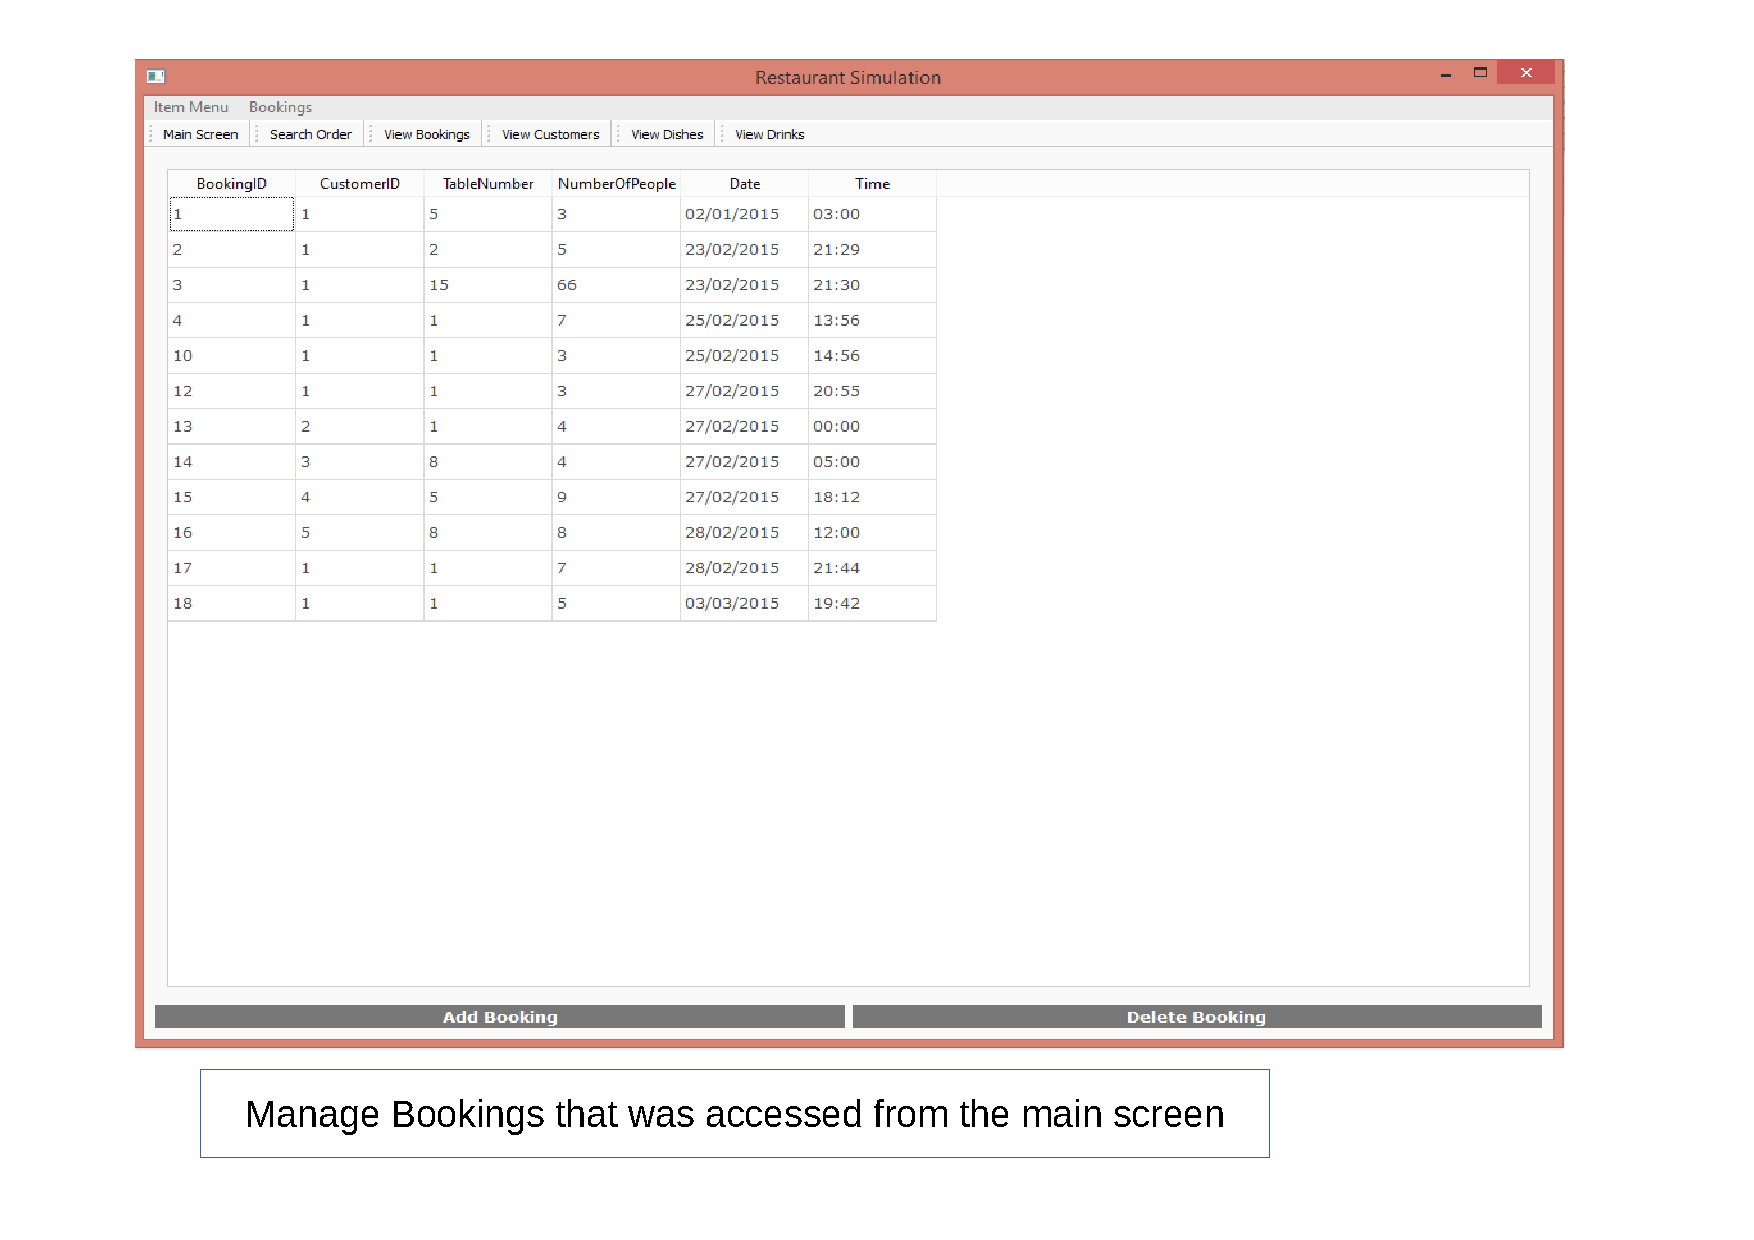
\includegraphics[height = 15cm]{./Maintenance/images/screen2}
    \caption{} \label{fig:screen2}
\end{figure}

\begin{figure}[H]
    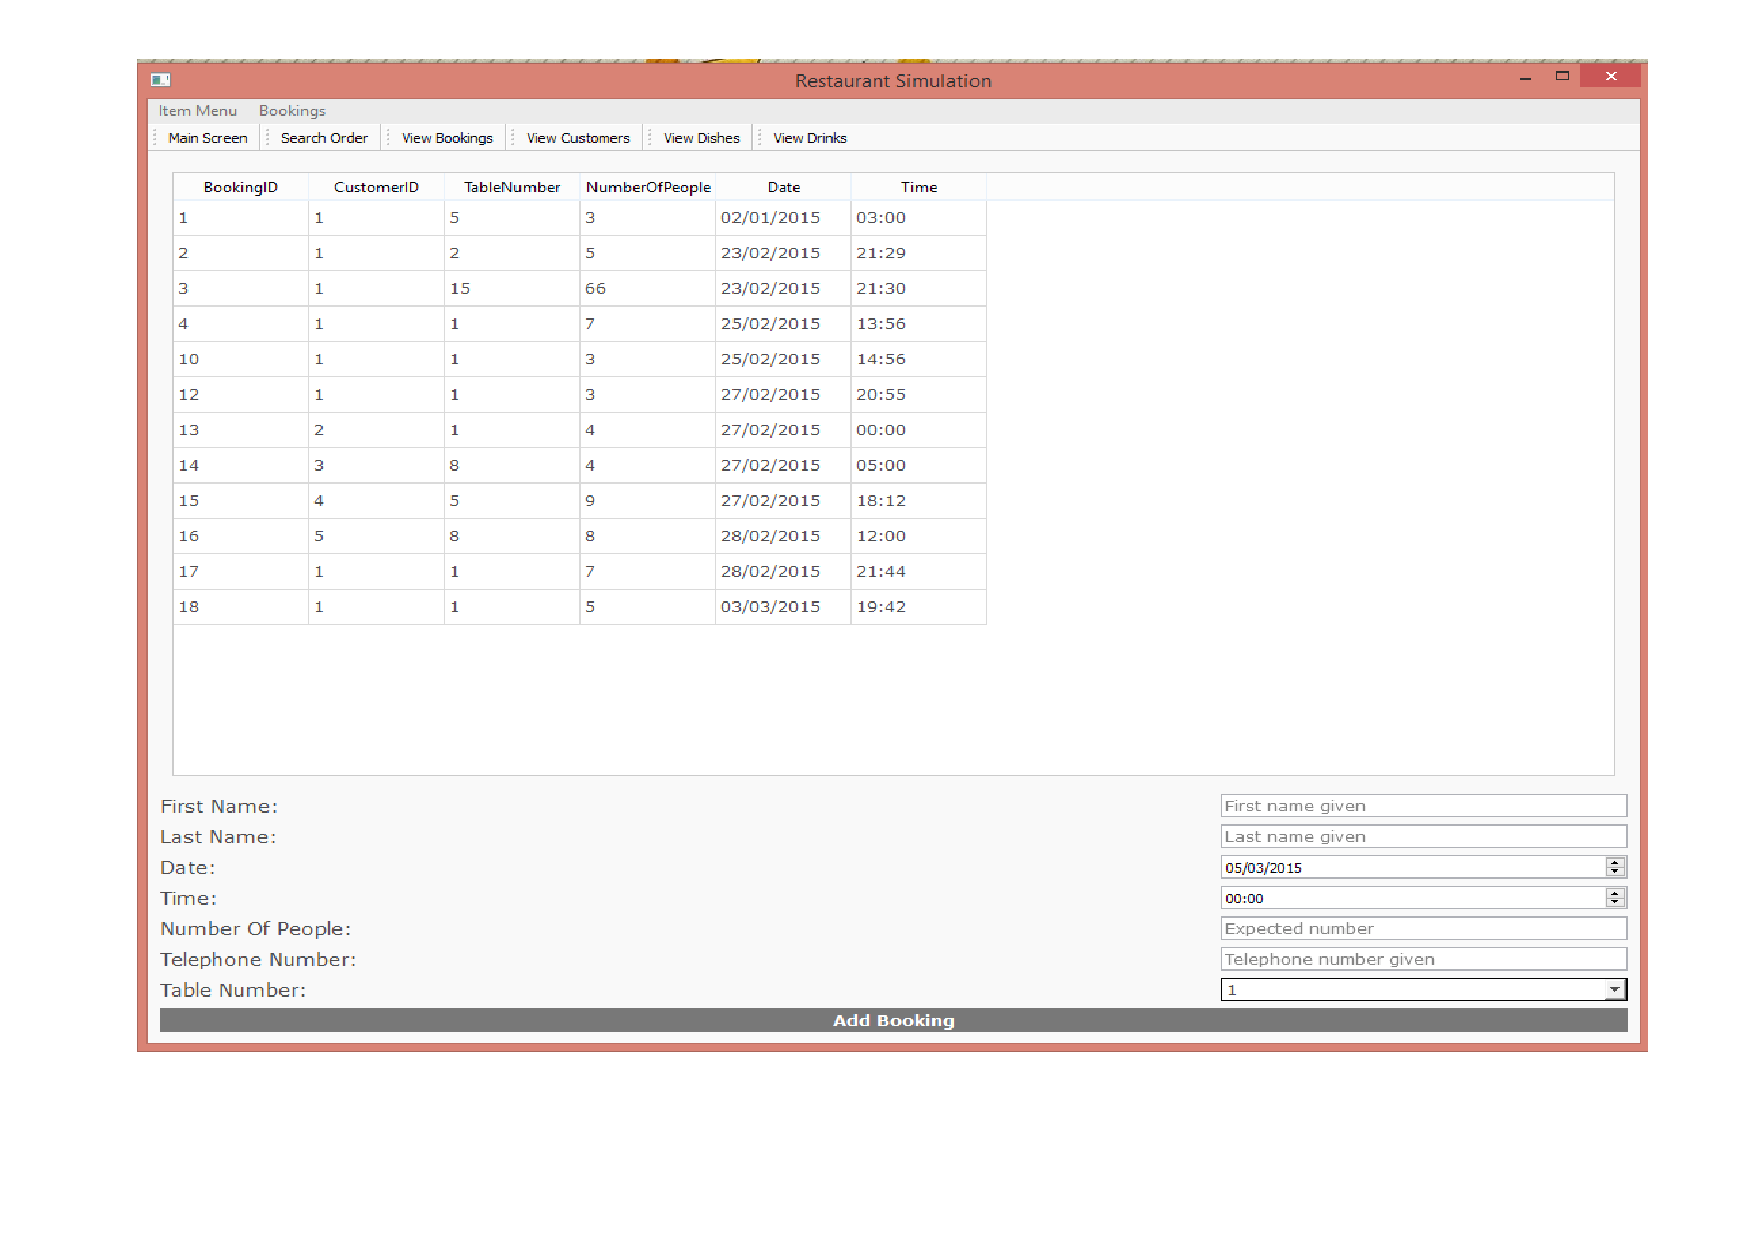
\includegraphics[height = 15cm]{./Maintenance/images/screen3}
    \caption{} \label{fig:screen3}
\end{figure}

\begin{figure}[H]
    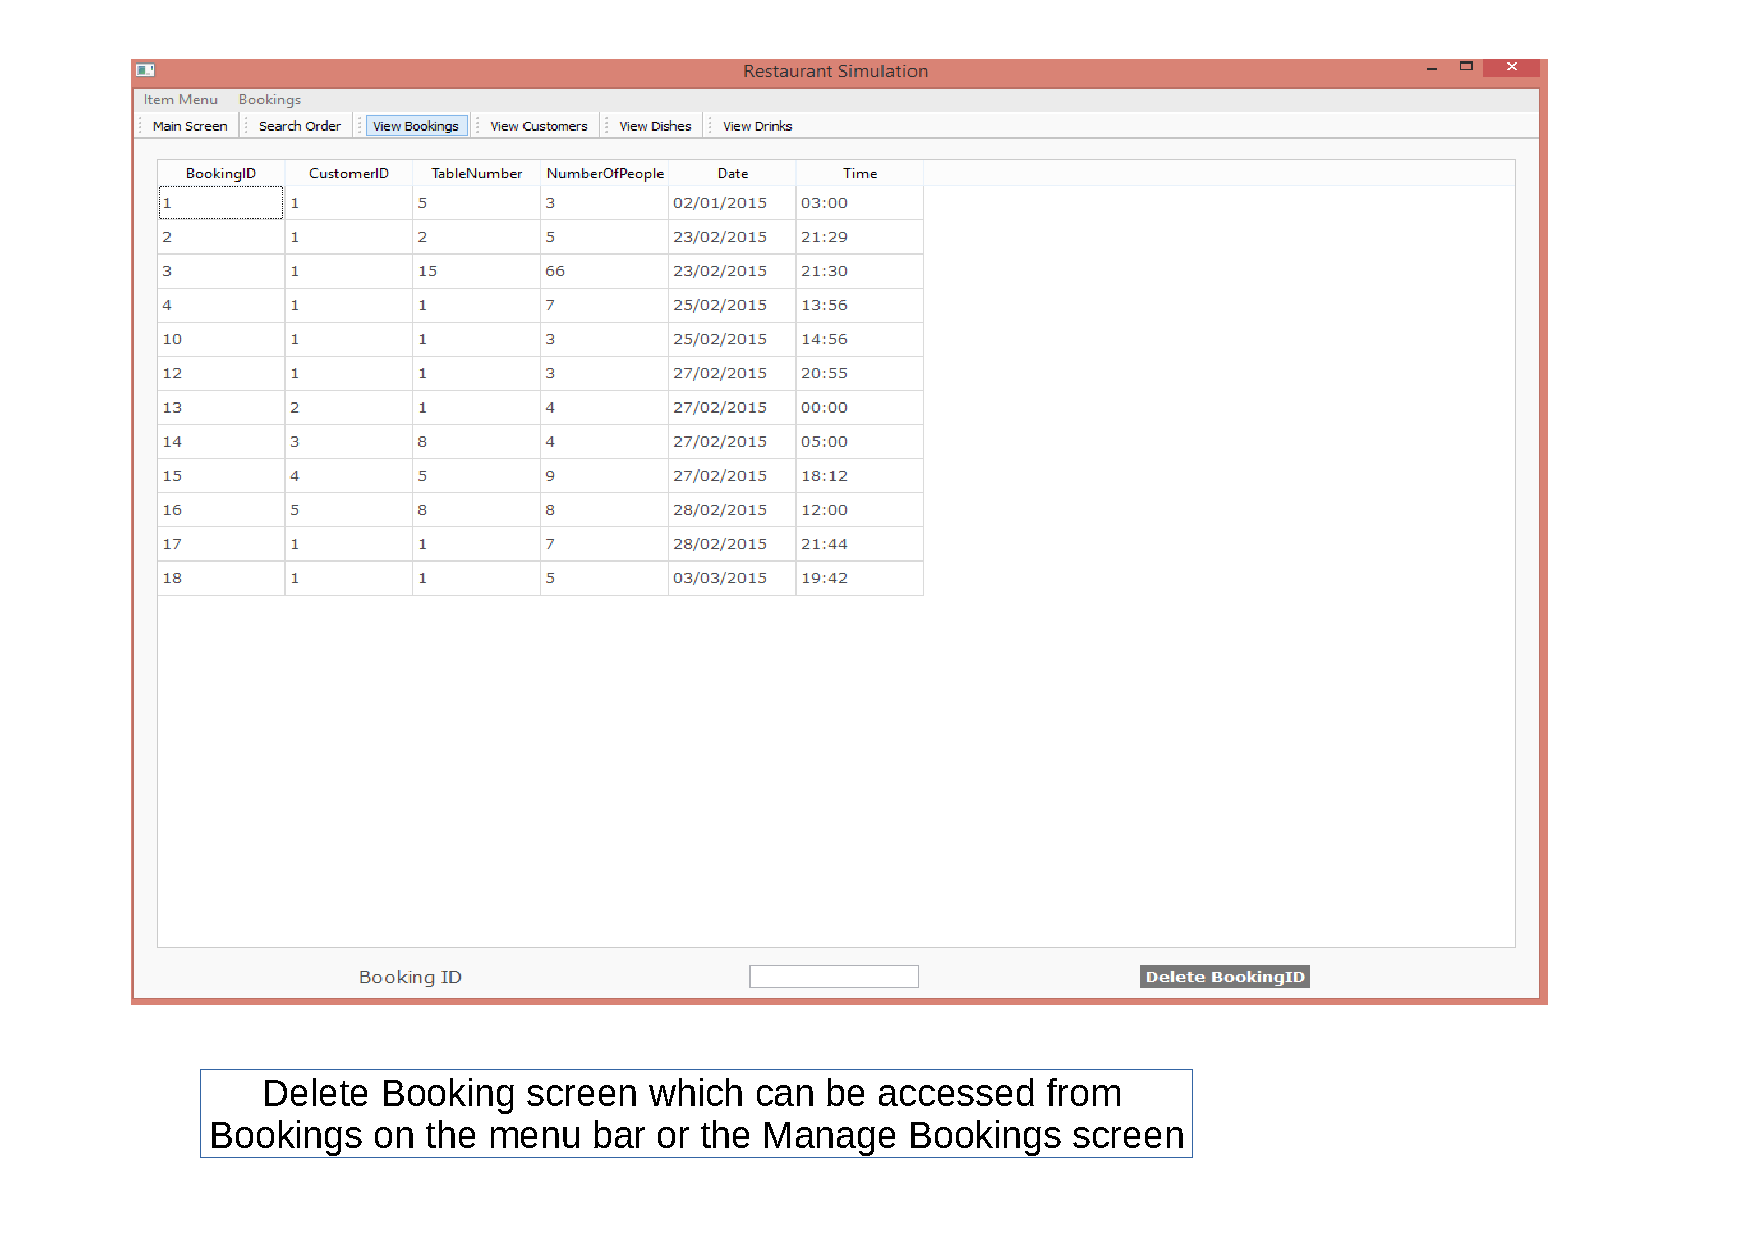
\includegraphics[height = 15cm]{./Maintenance/images/screen4}
    \caption{} \label{fig:screen4}
\end{figure}

\begin{figure}[H]
    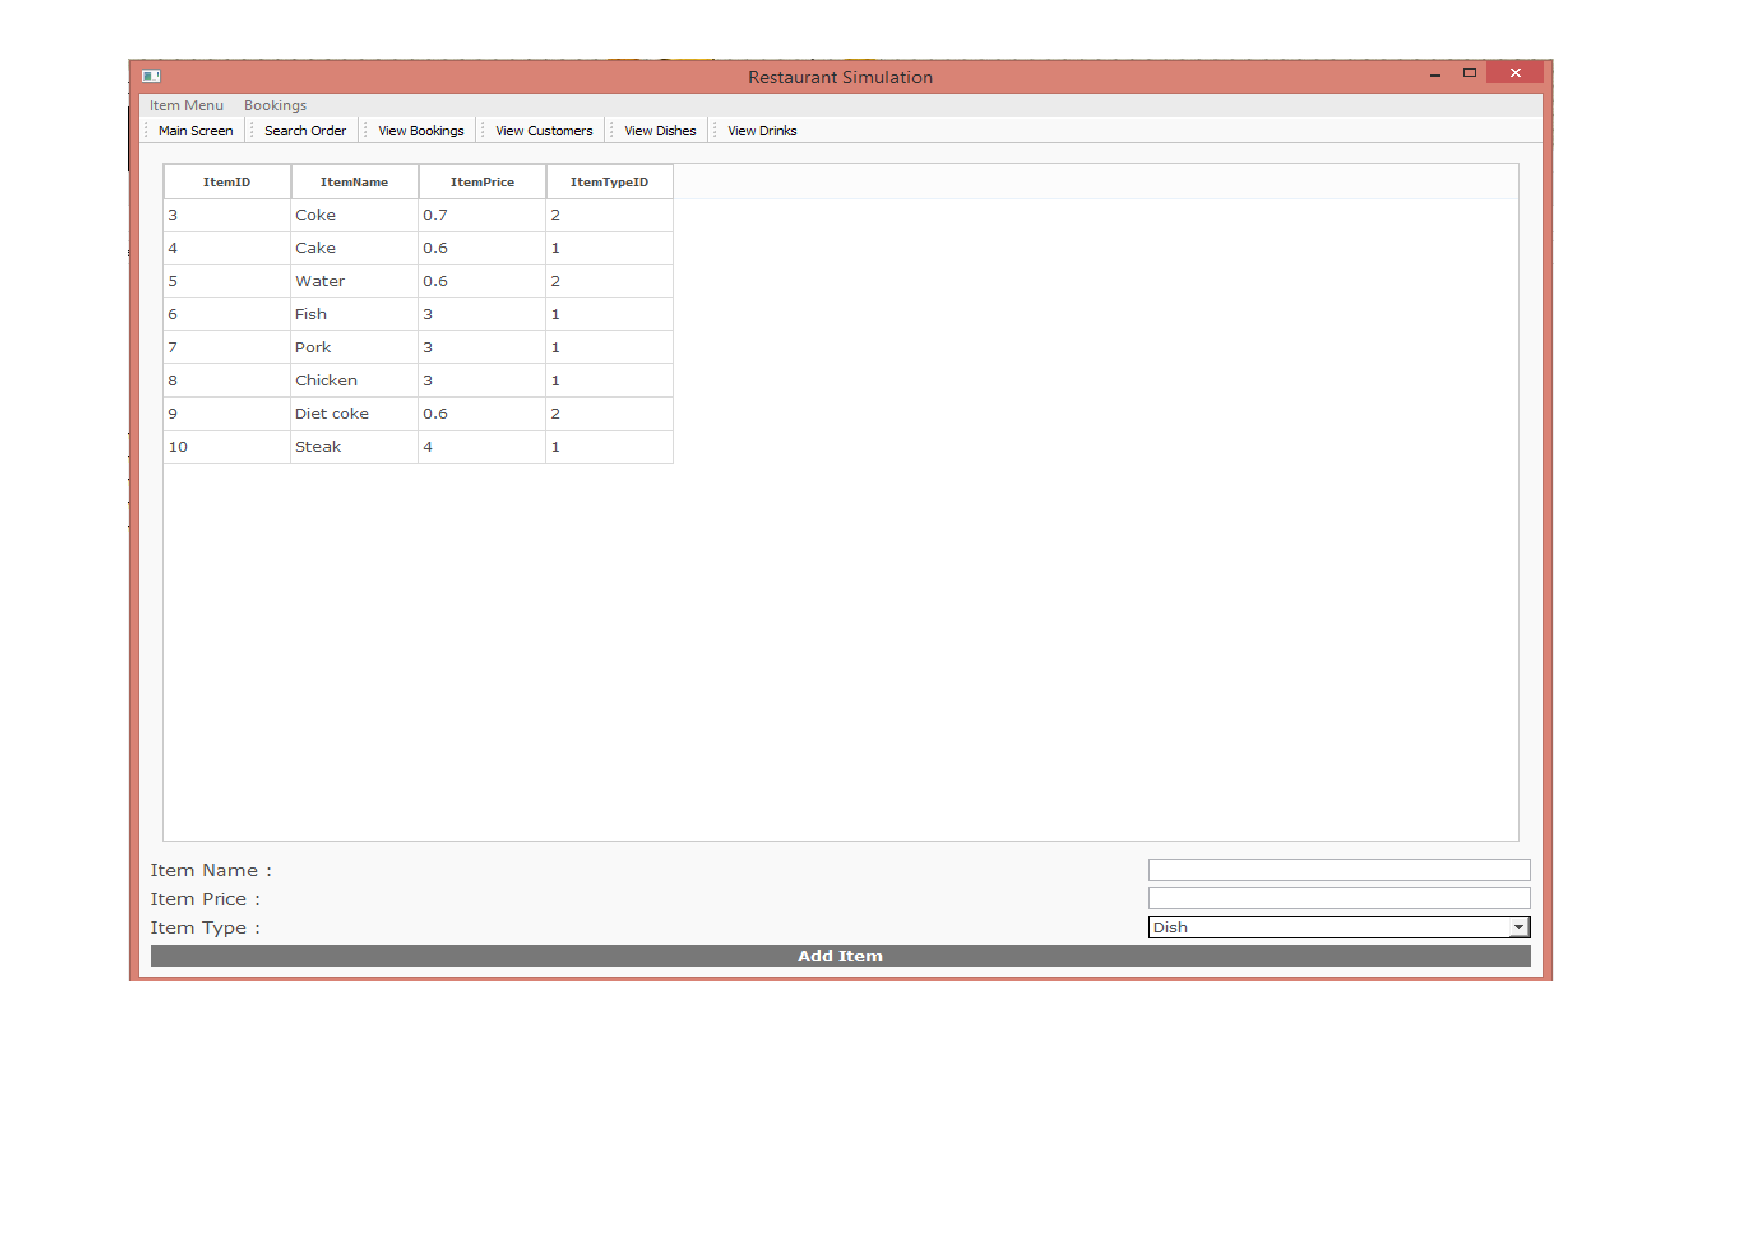
\includegraphics[height = 15cm]{./Maintenance/images/screen5}
    \caption{} \label{fig:screen5}
\end{figure}

\begin{figure}[H]
    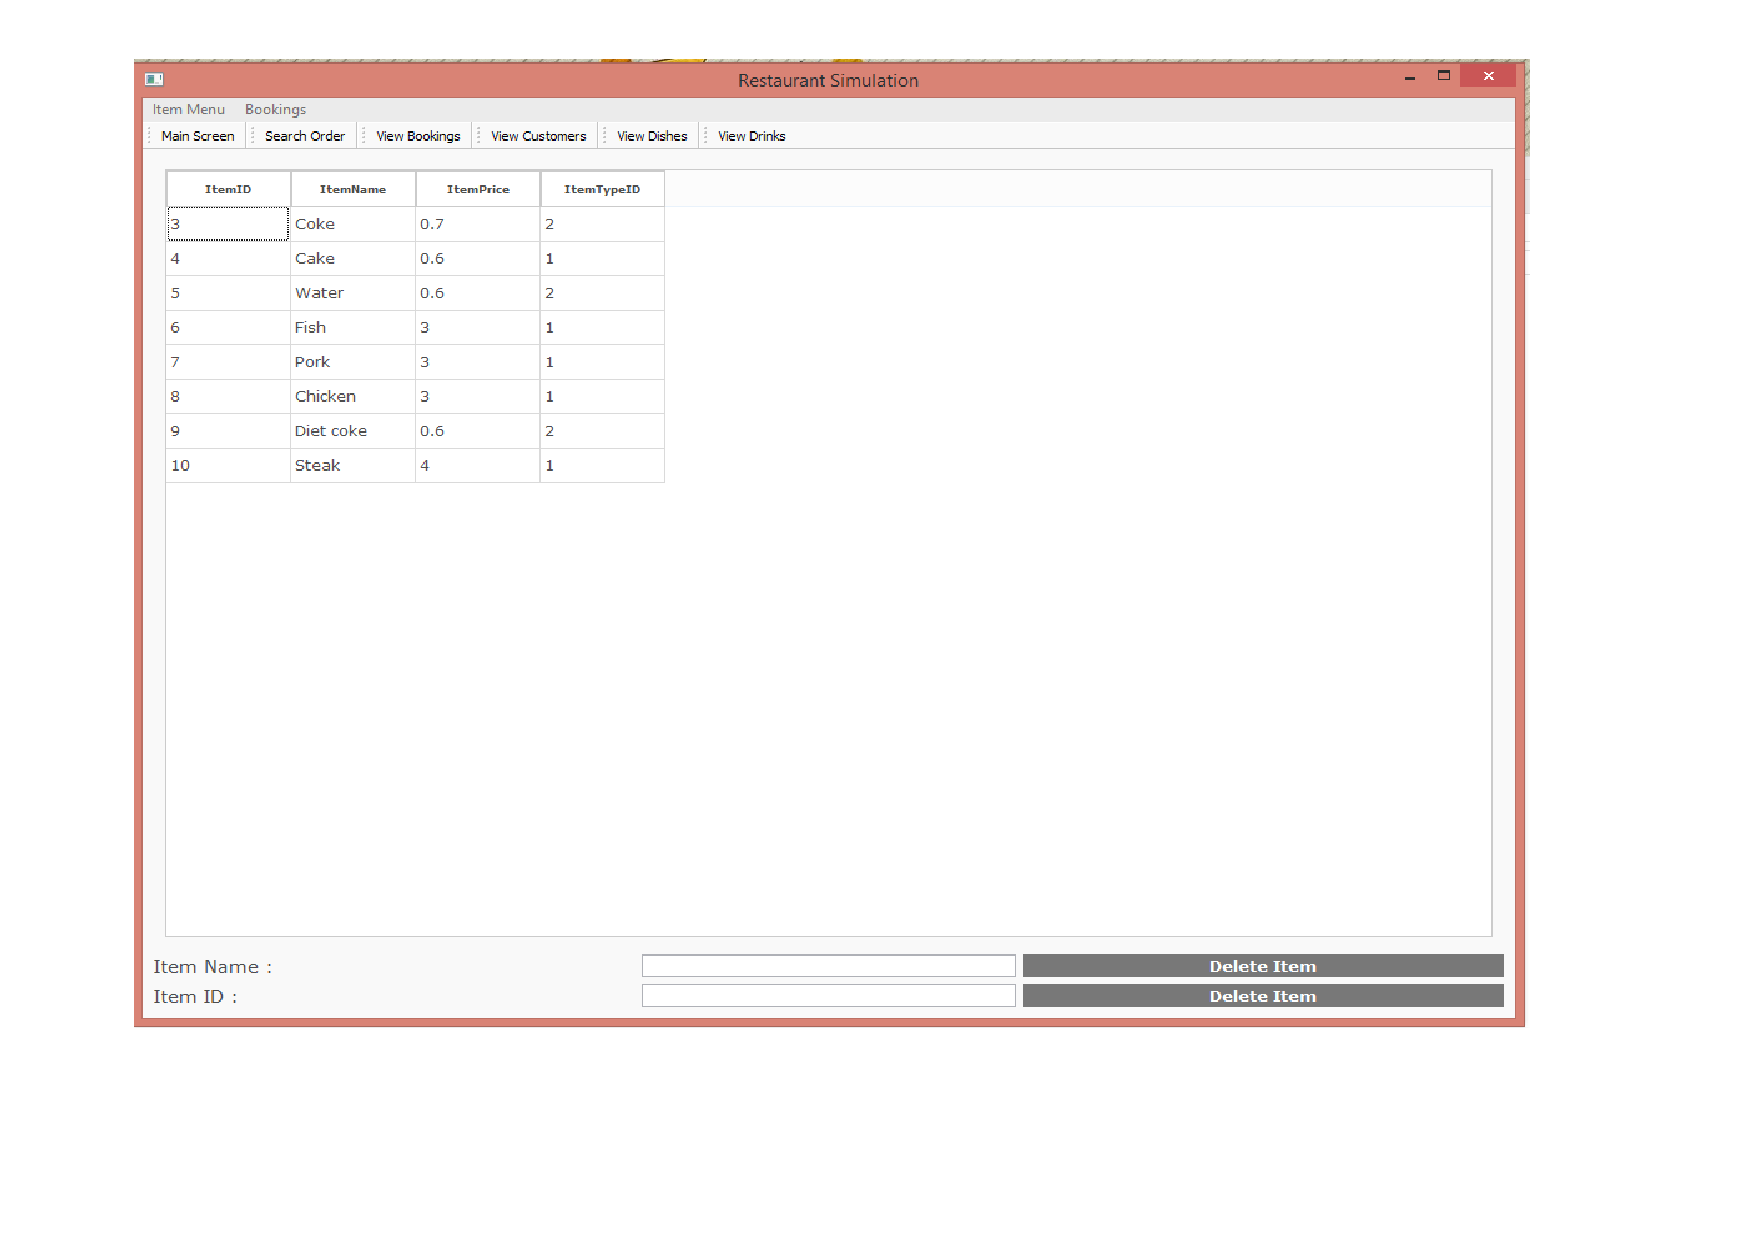
\includegraphics[height = 15cm]{./Maintenance/images/screen6}
    \caption{} \label{fig:screen6}
\end{figure}

\begin{figure}[H]
    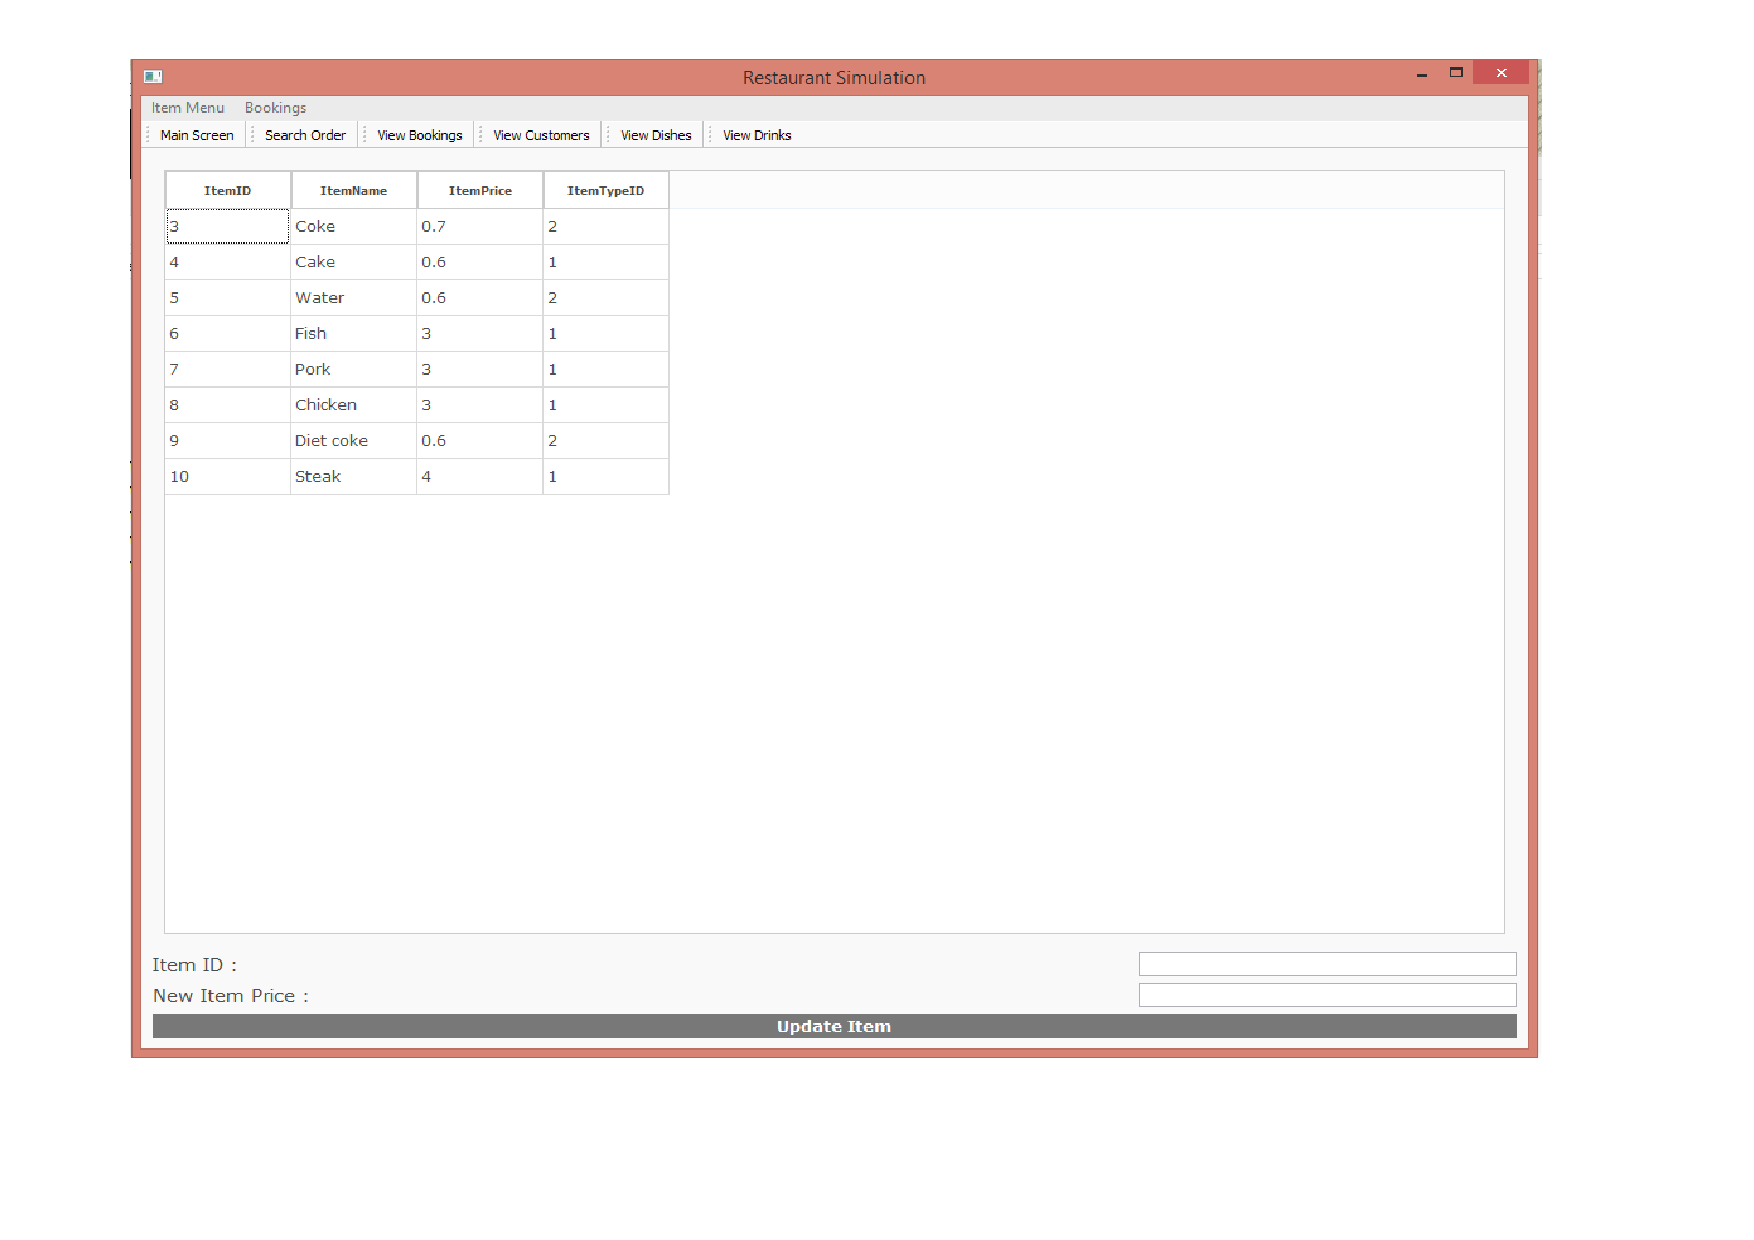
\includegraphics[height = 15cm]{./Maintenance/images/screen7}
    \caption{} \label{fig:screen7}
\end{figure}

\begin{figure}[H]
    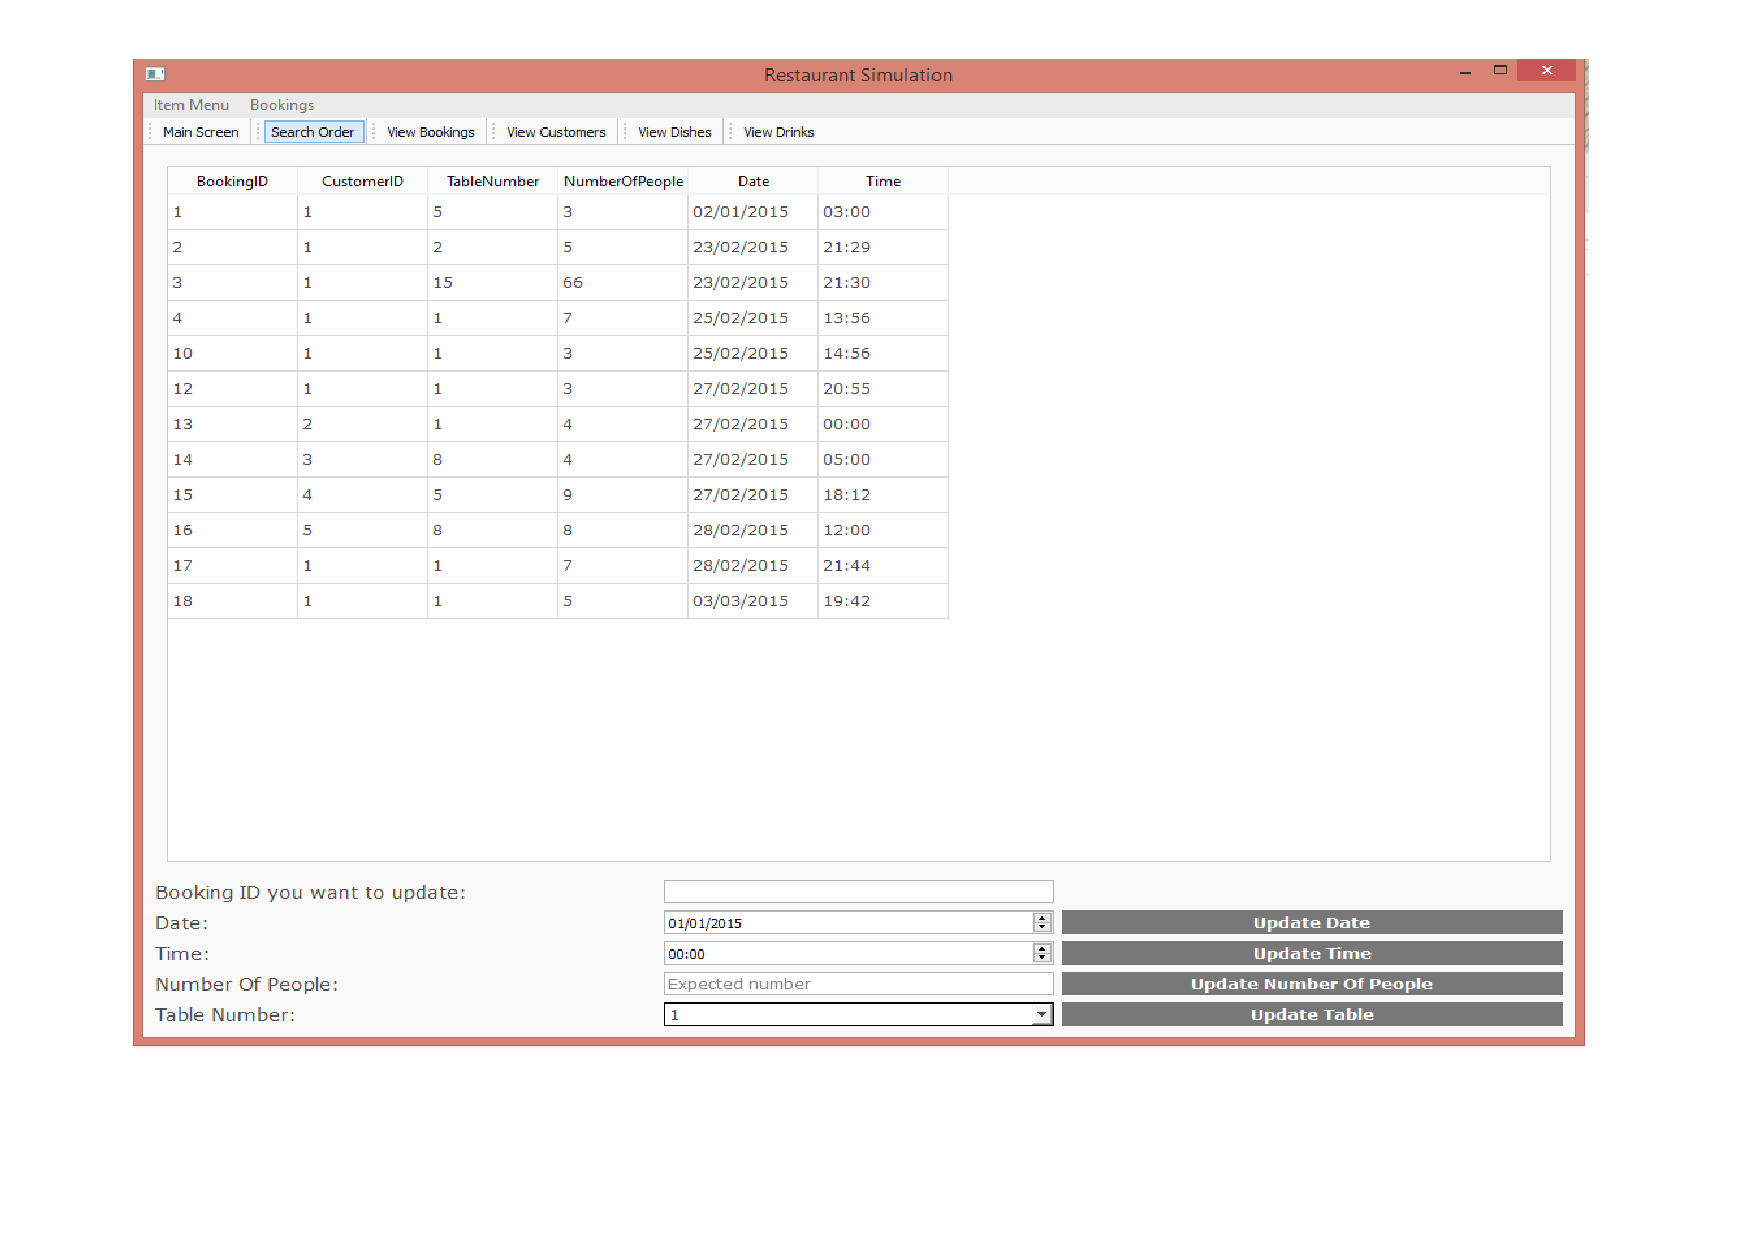
\includegraphics[height = 15cm]{./Maintenance/images/screen8}
    \caption{} \label{fig:screen8}
\end{figure}

\begin{figure}[H]
    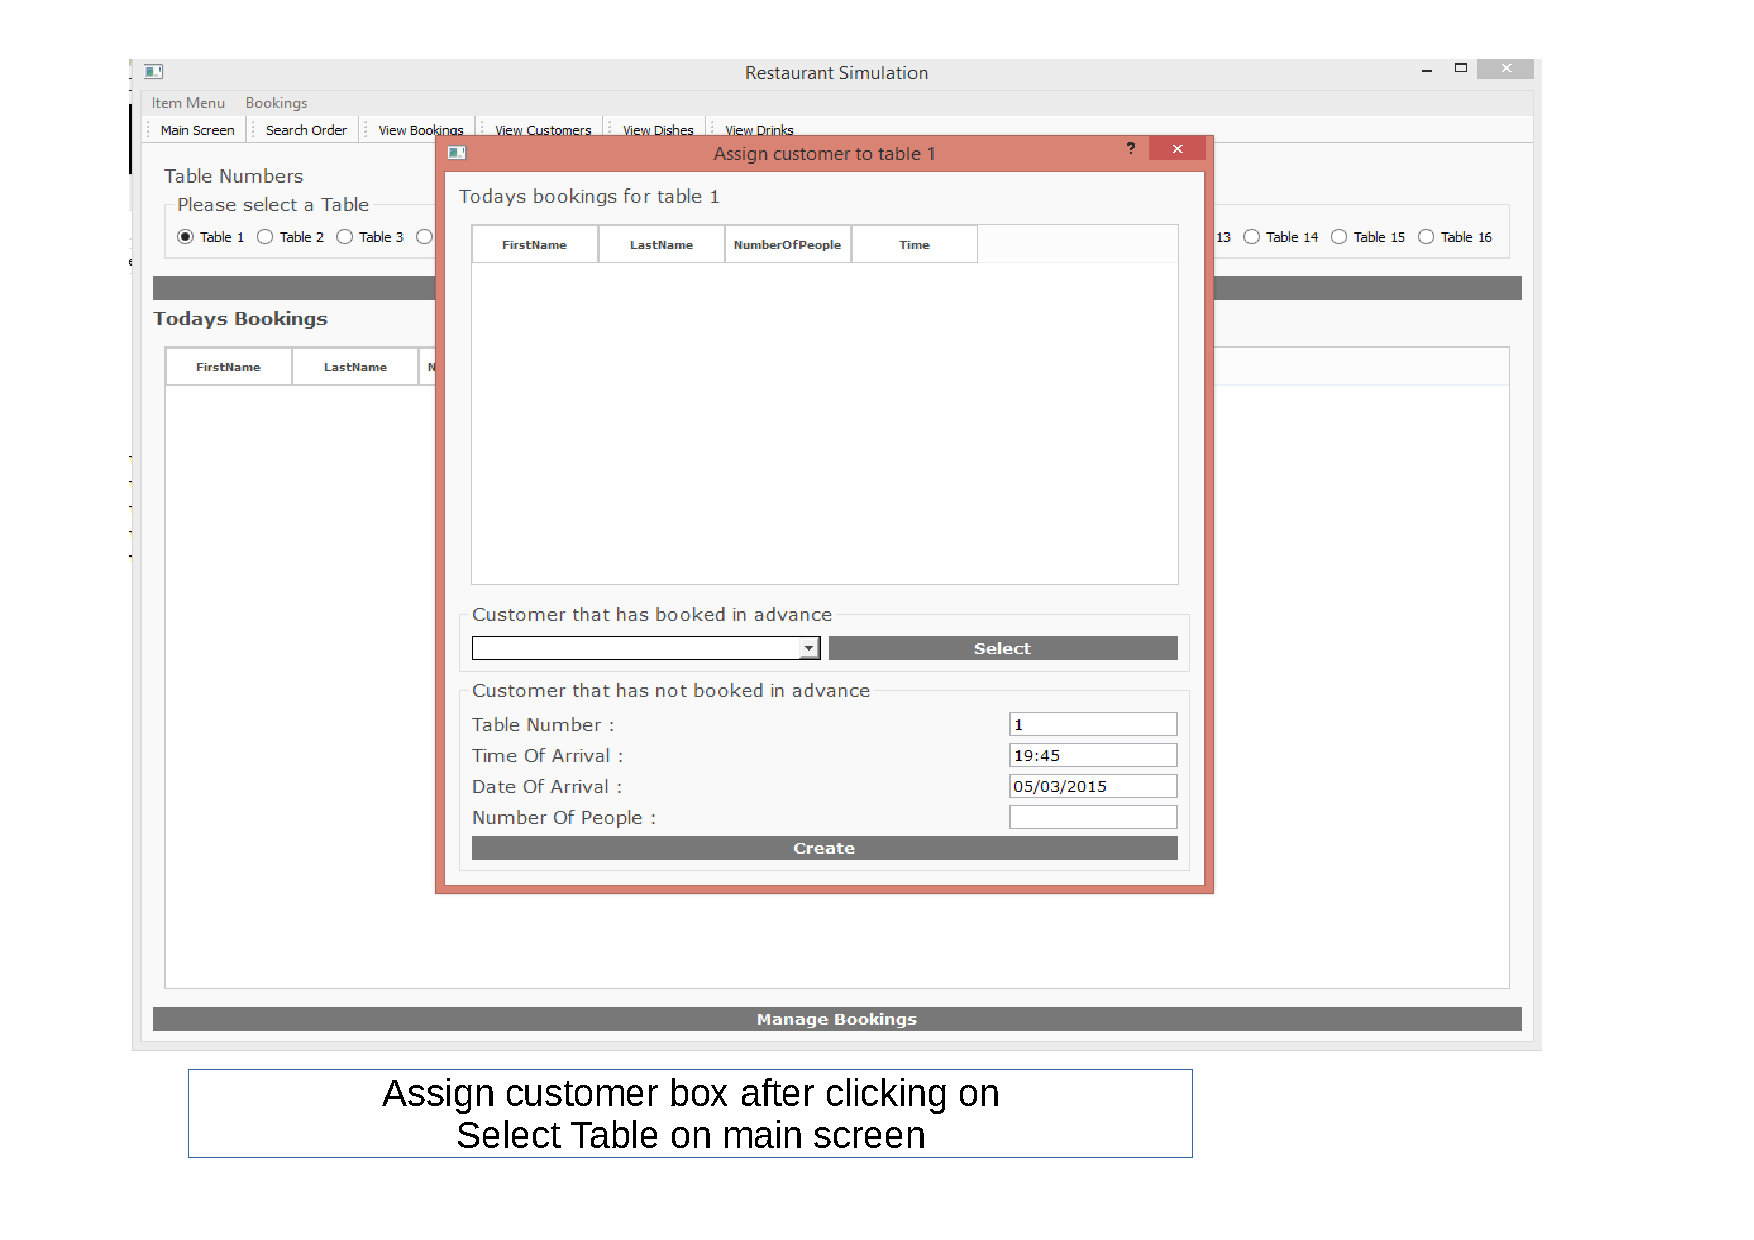
\includegraphics[height = 15cm]{./Maintenance/images/screen9}
    \caption{} \label{fig:screen9}
\end{figure}

\begin{figure}[H]
    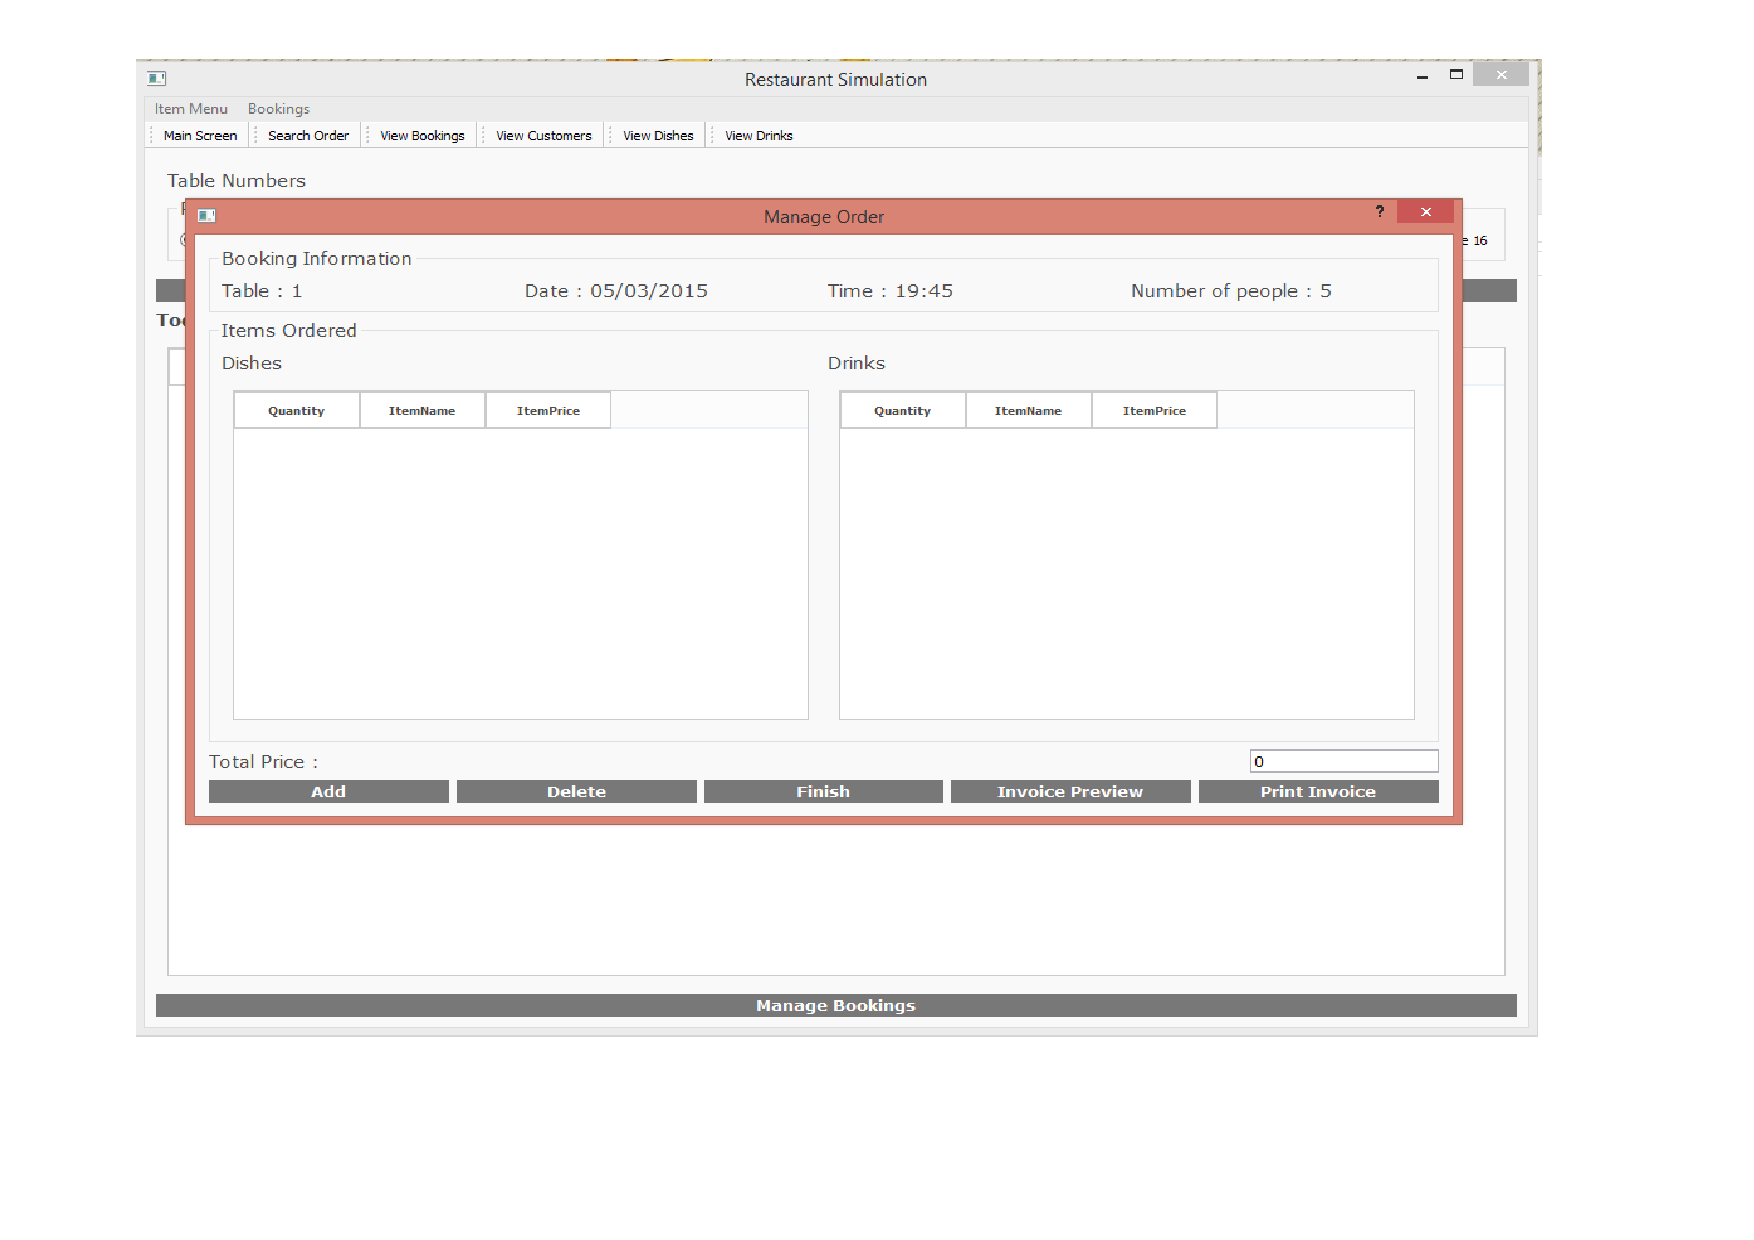
\includegraphics[height = 15cm]{./Maintenance/images/screen10}
    \caption{} \label{fig:screen10}
\end{figure}

\begin{figure}[H]
    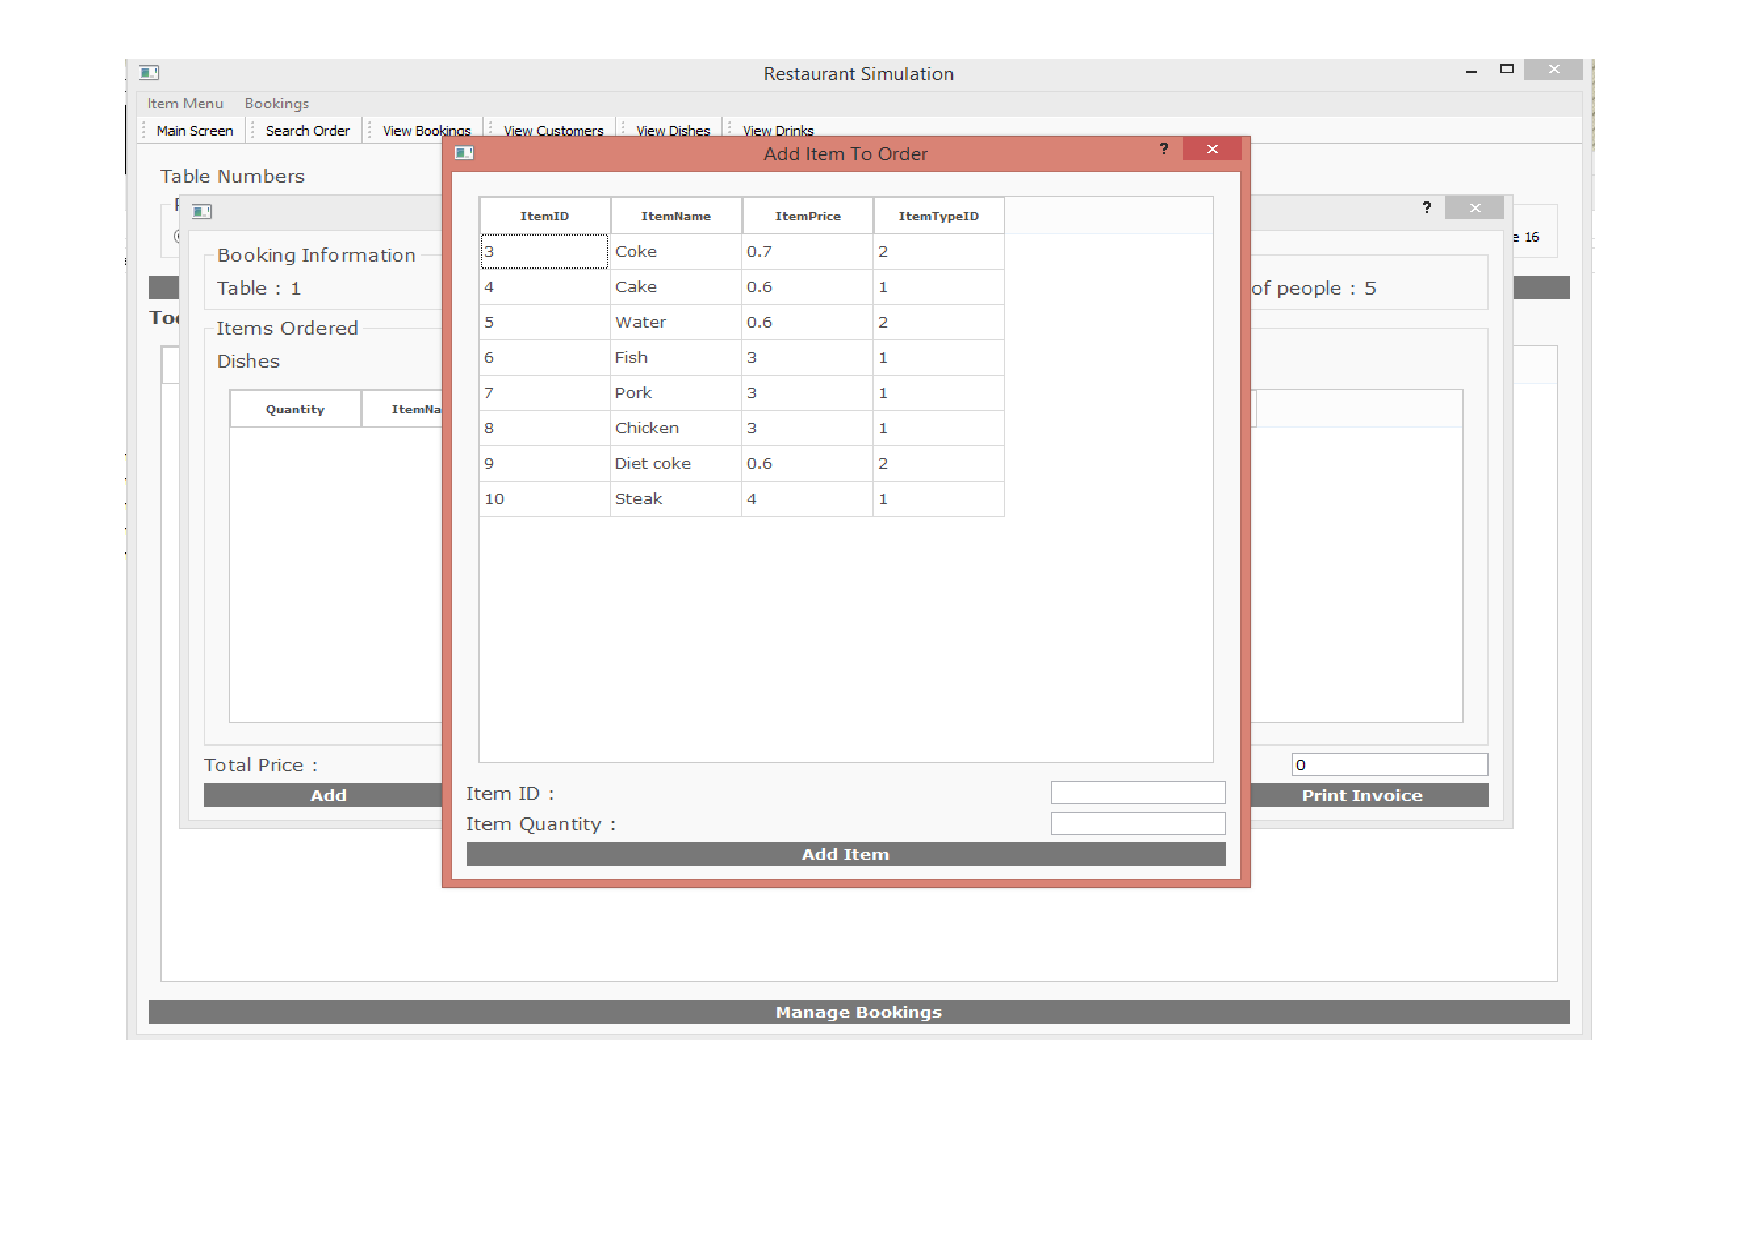
\includegraphics[height = 15cm]{./Maintenance/images/screen11}
    \caption{} \label{fig:screen11}
\end{figure}

\begin{figure}[H]
    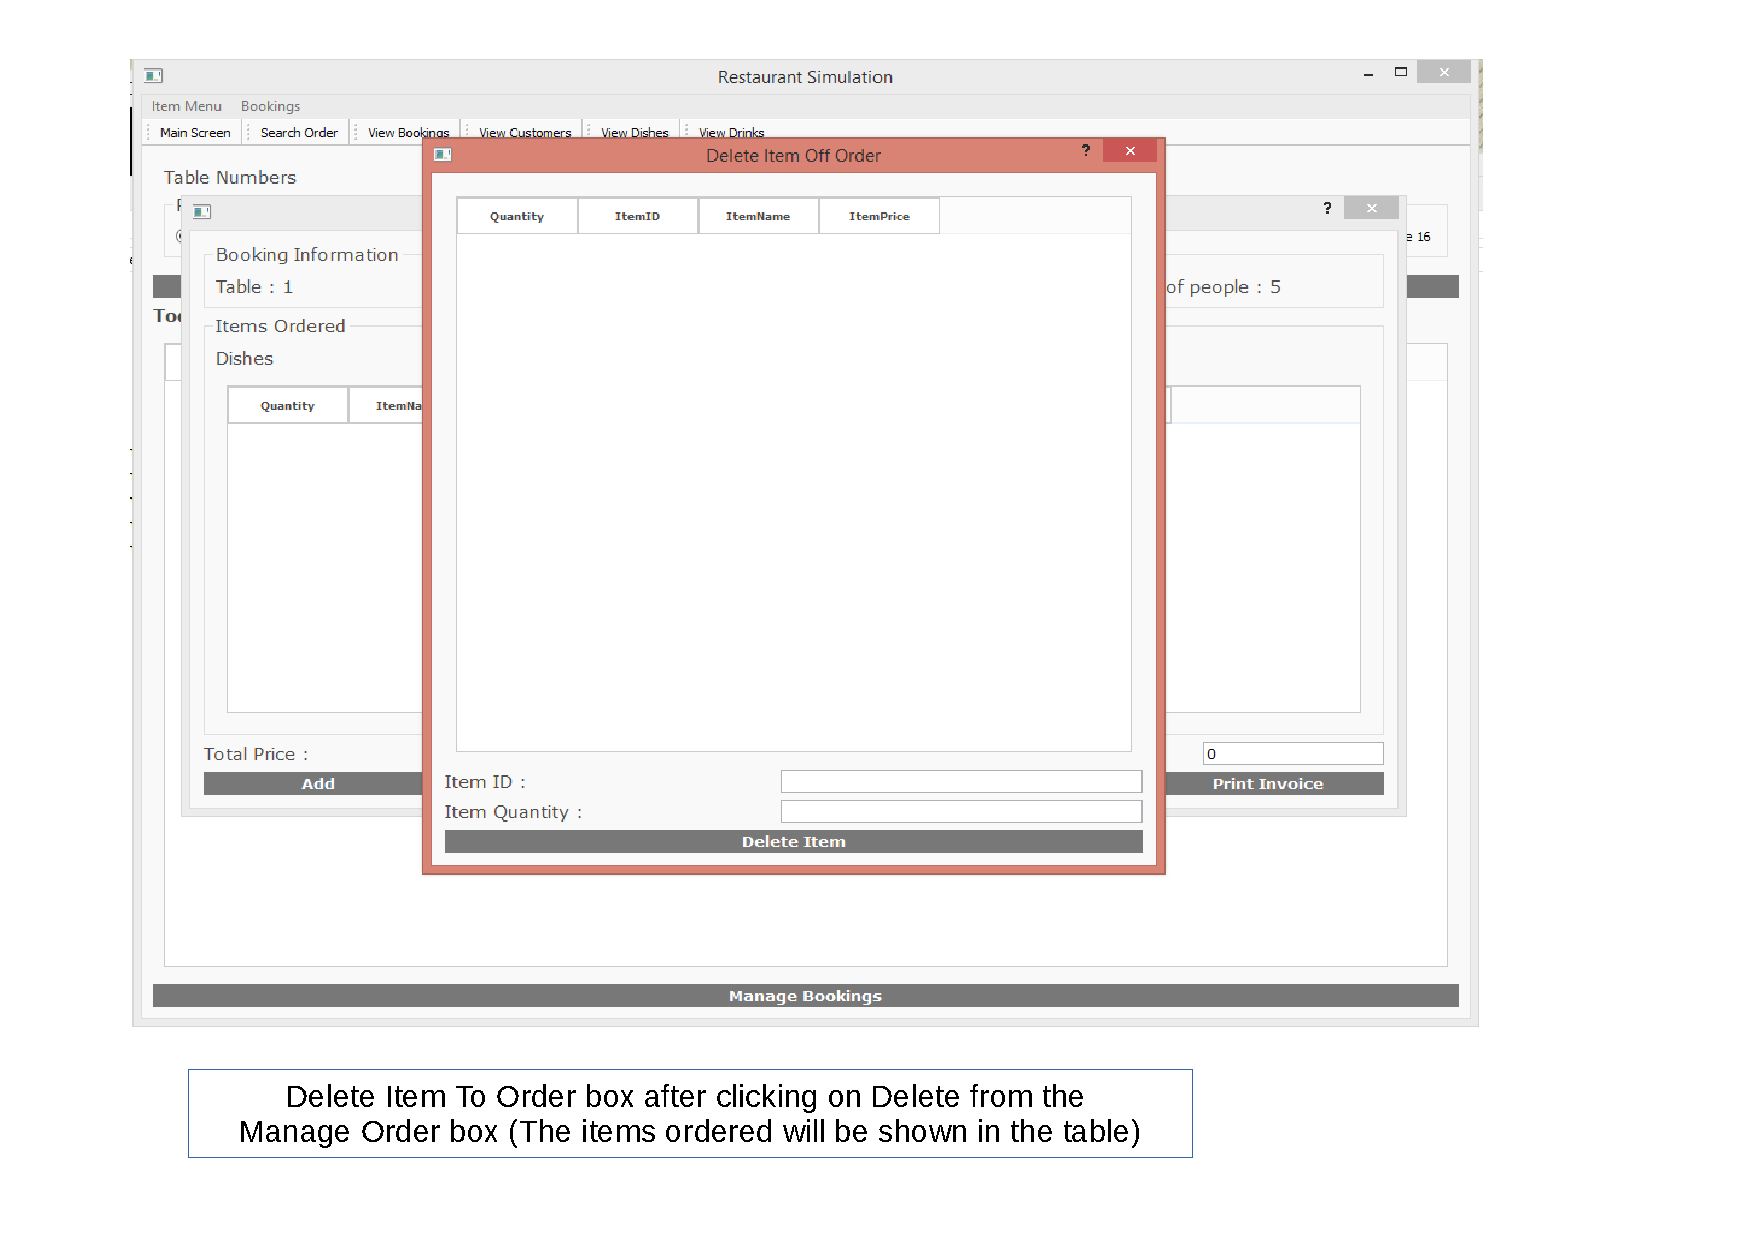
\includegraphics[height = 15cm]{./Maintenance/images/screen12}
    \caption{} \label{fig:screen12}
\end{figure}

\begin{figure}[H]
    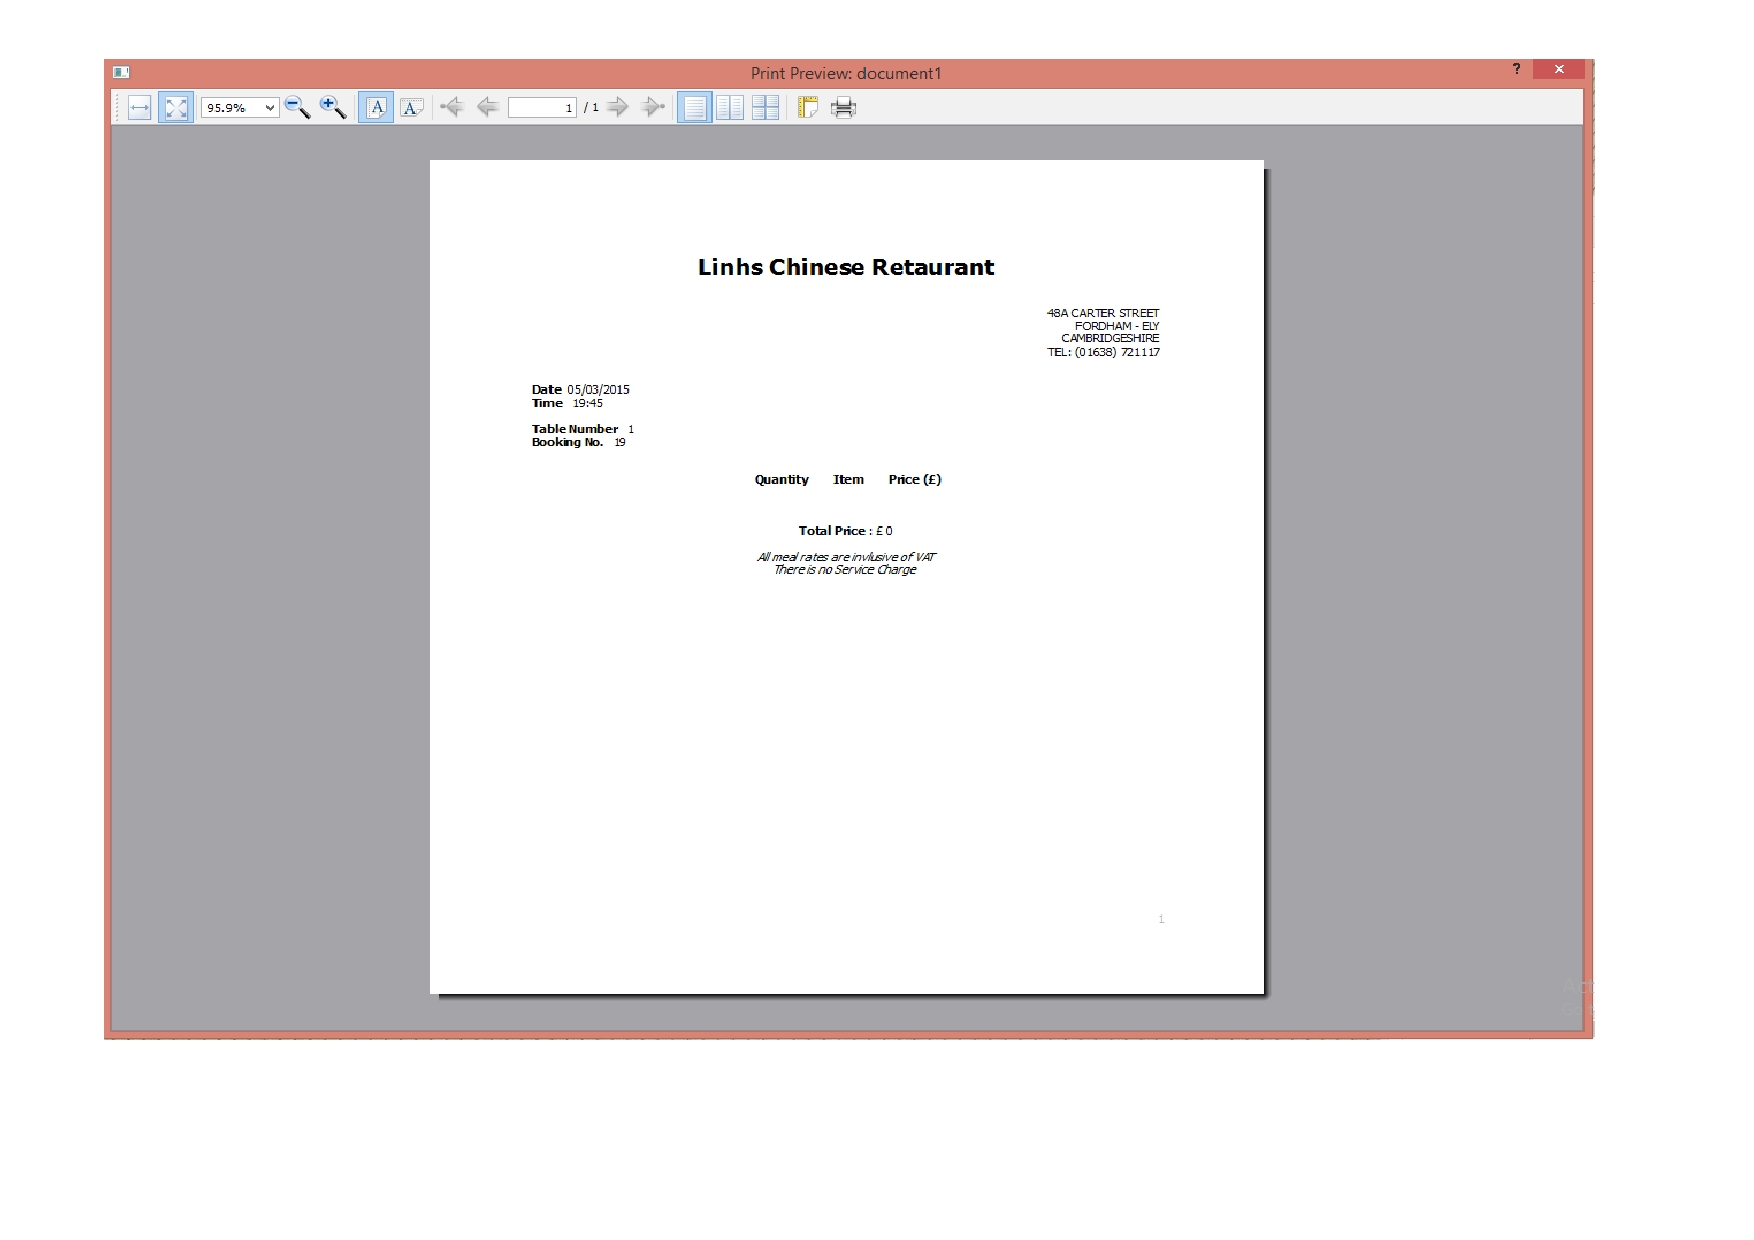
\includegraphics[height = 15cm]{./Maintenance/images/screen13}
    \caption{} \label{fig:screen13}
\end{figure}

\begin{figure}[H]
    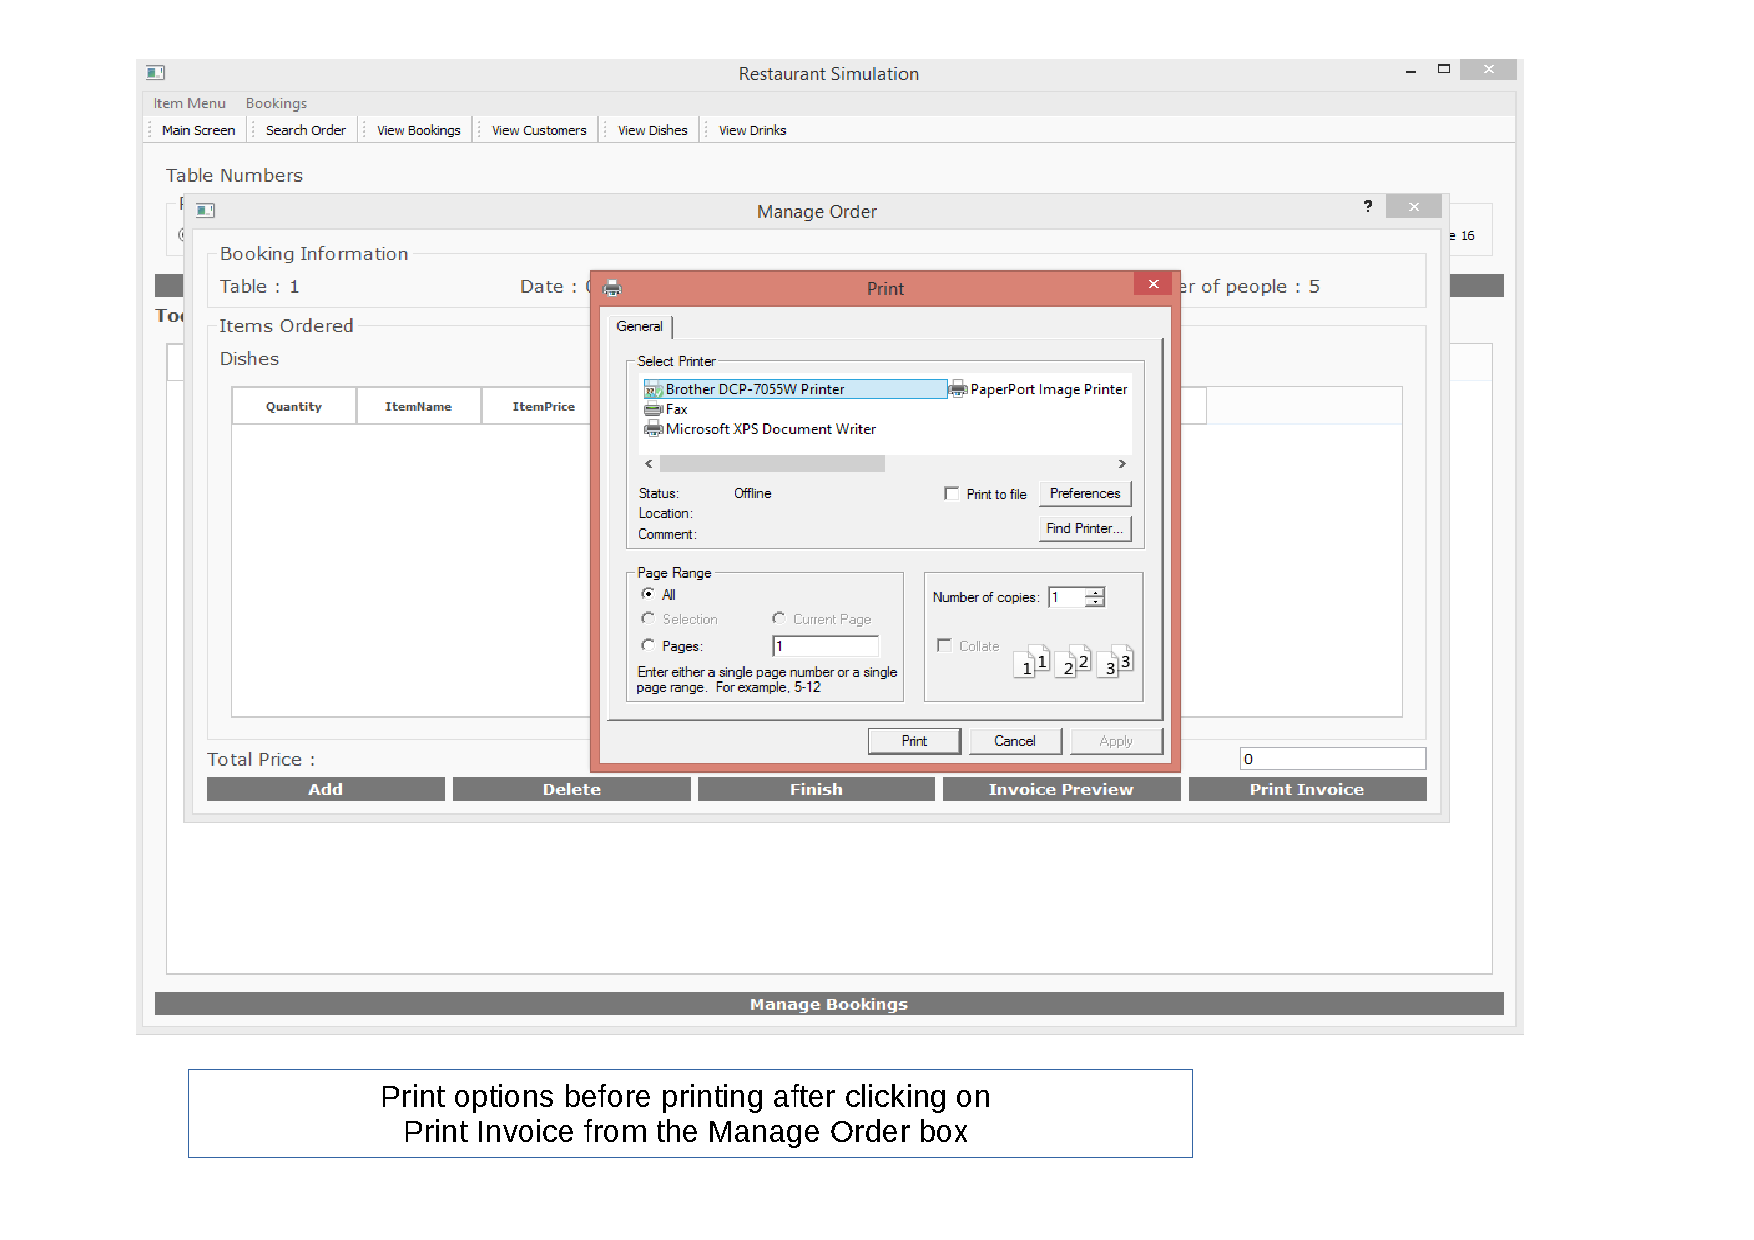
\includegraphics[height = 15cm]{./Maintenance/images/screen14}
    \caption{} \label{fig:screen14}
\end{figure}

\begin{figure}[H]
    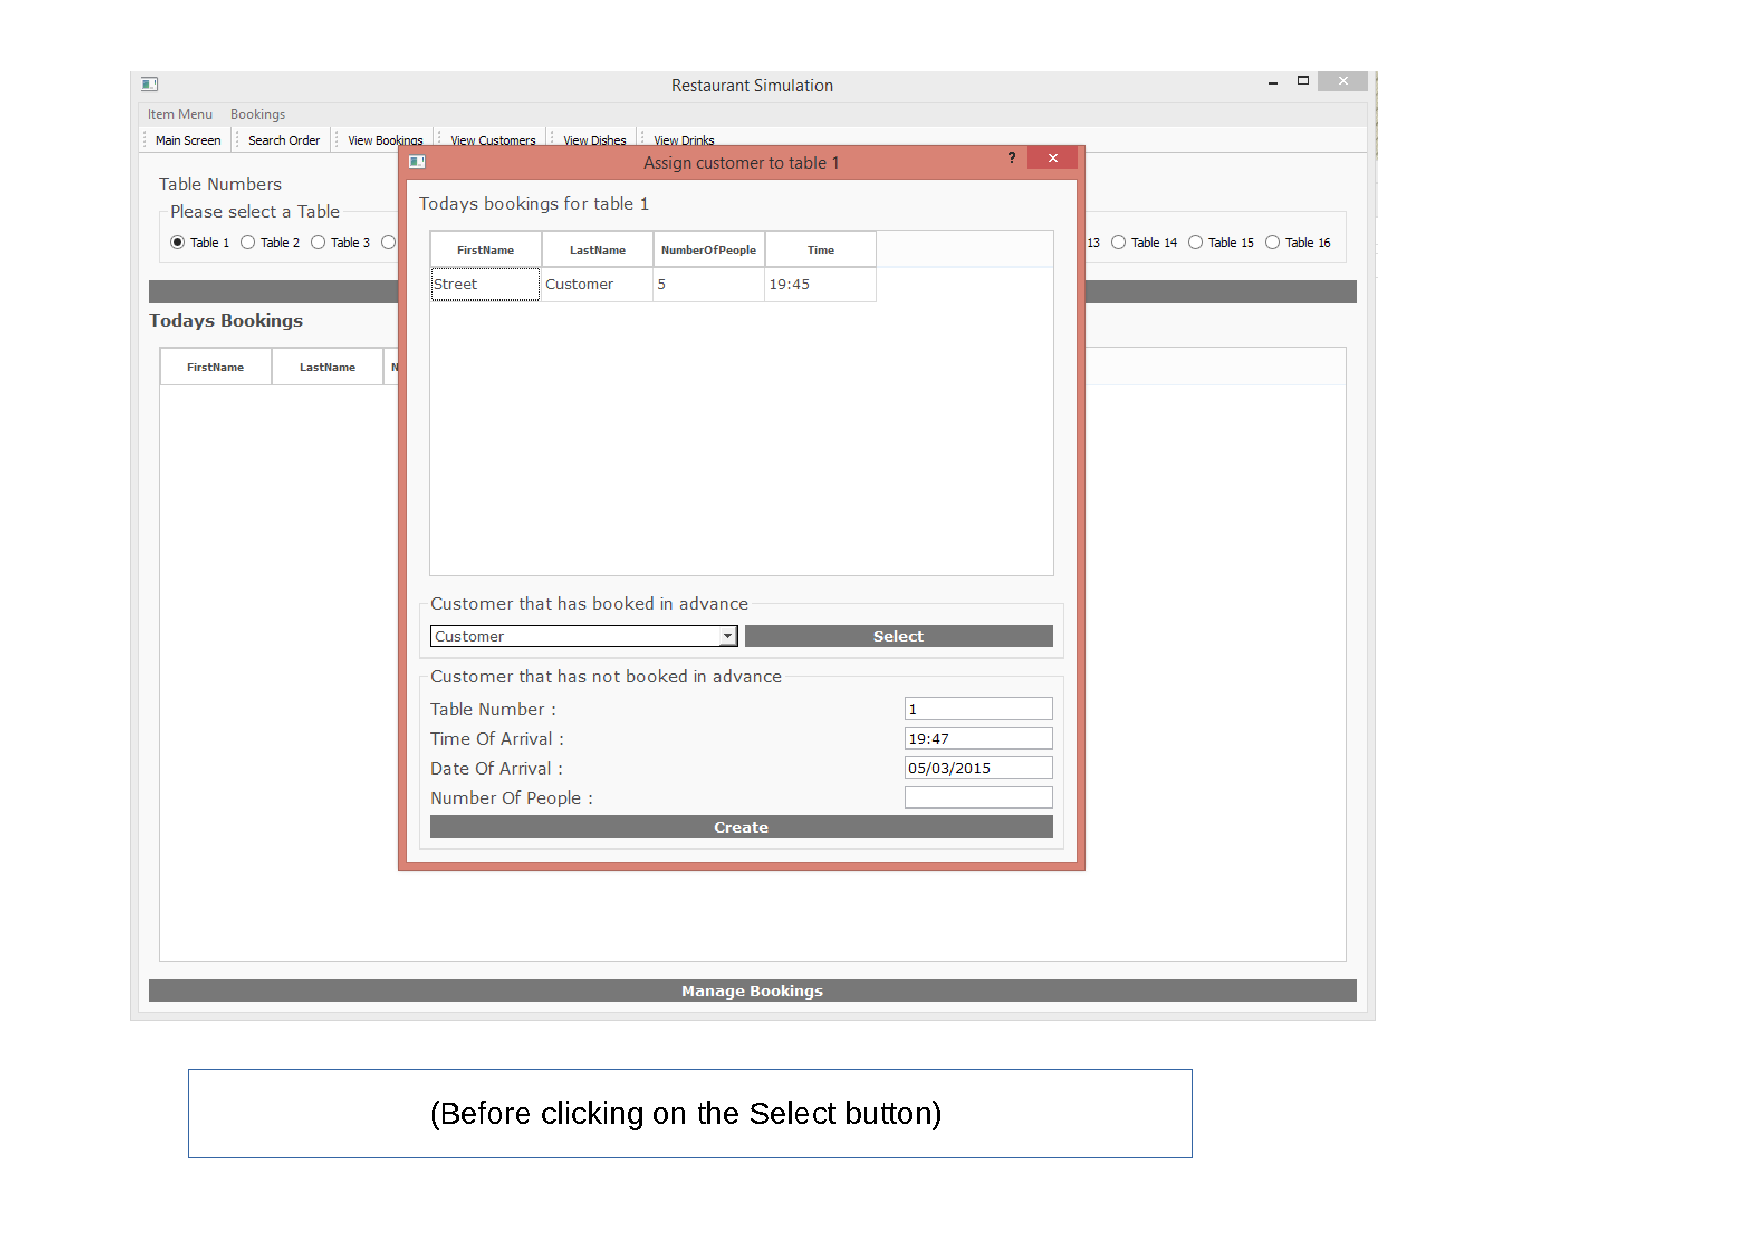
\includegraphics[height = 15cm]{./Maintenance/images/screen15}
    \caption{} \label{fig:screen15}
\end{figure}

\begin{figure}[H]
    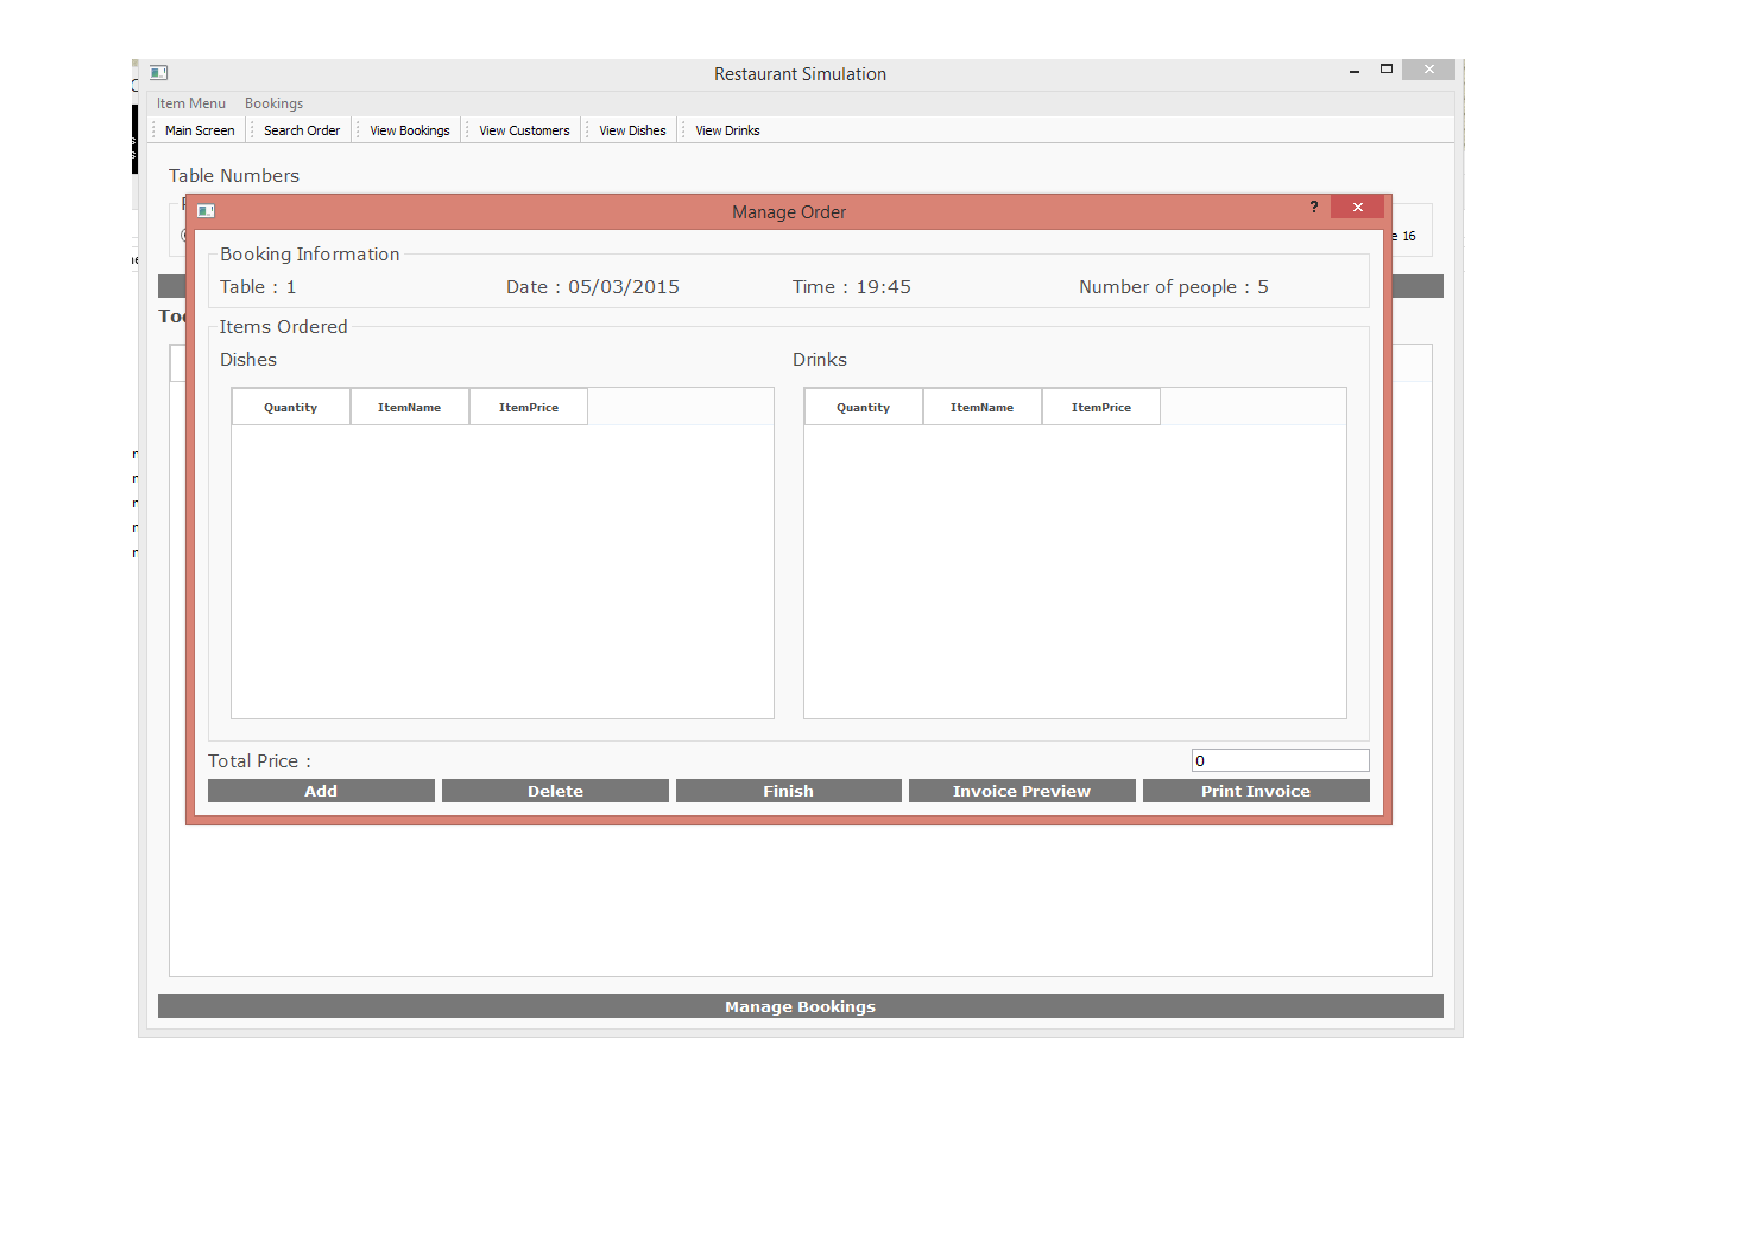
\includegraphics[height = 15cm]{./Maintenance/images/screen16}
    \caption{} \label{fig:screen16}
\end{figure}

\begin{figure}[H]
    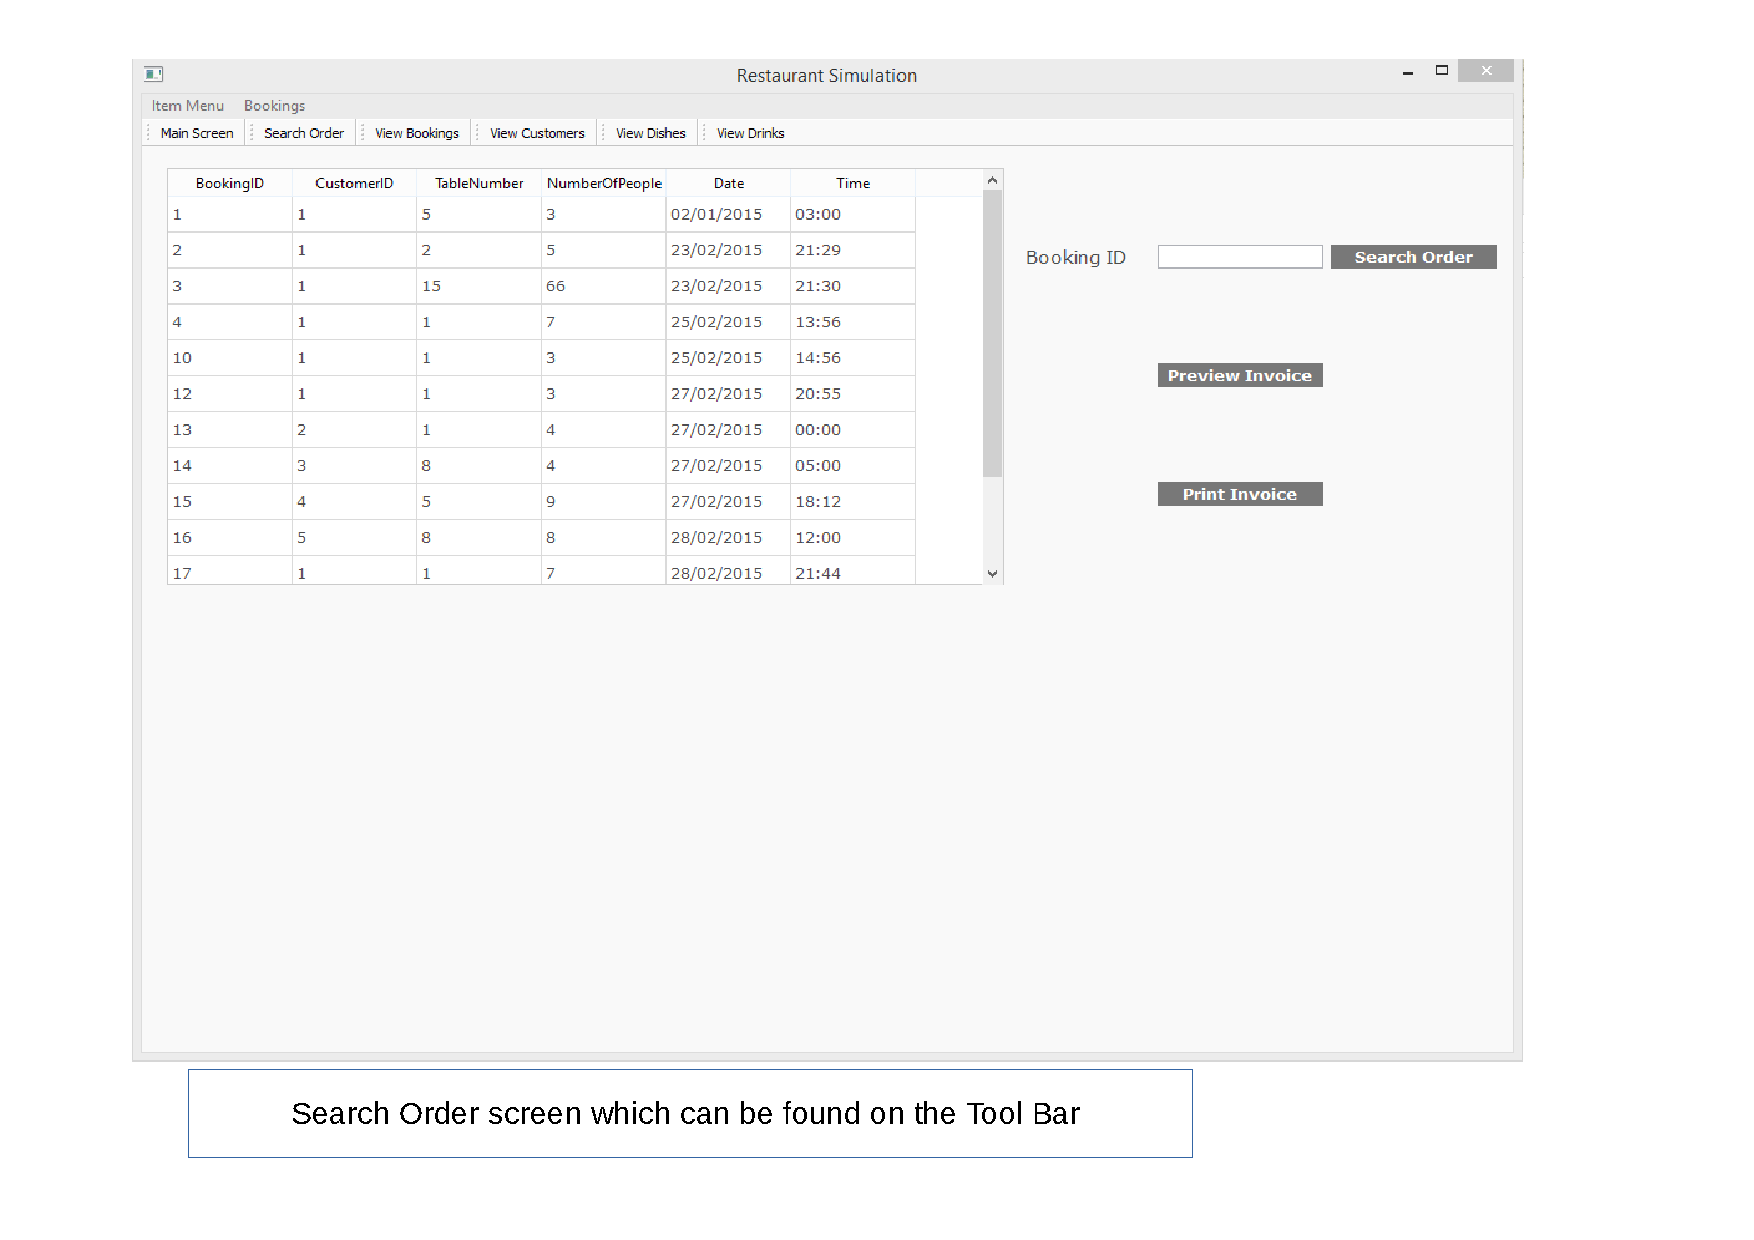
\includegraphics[height = 15cm]{./Maintenance/images/screen17}
    \caption{} \label{fig:screen17}
\end{figure}

\begin{figure}[H]
    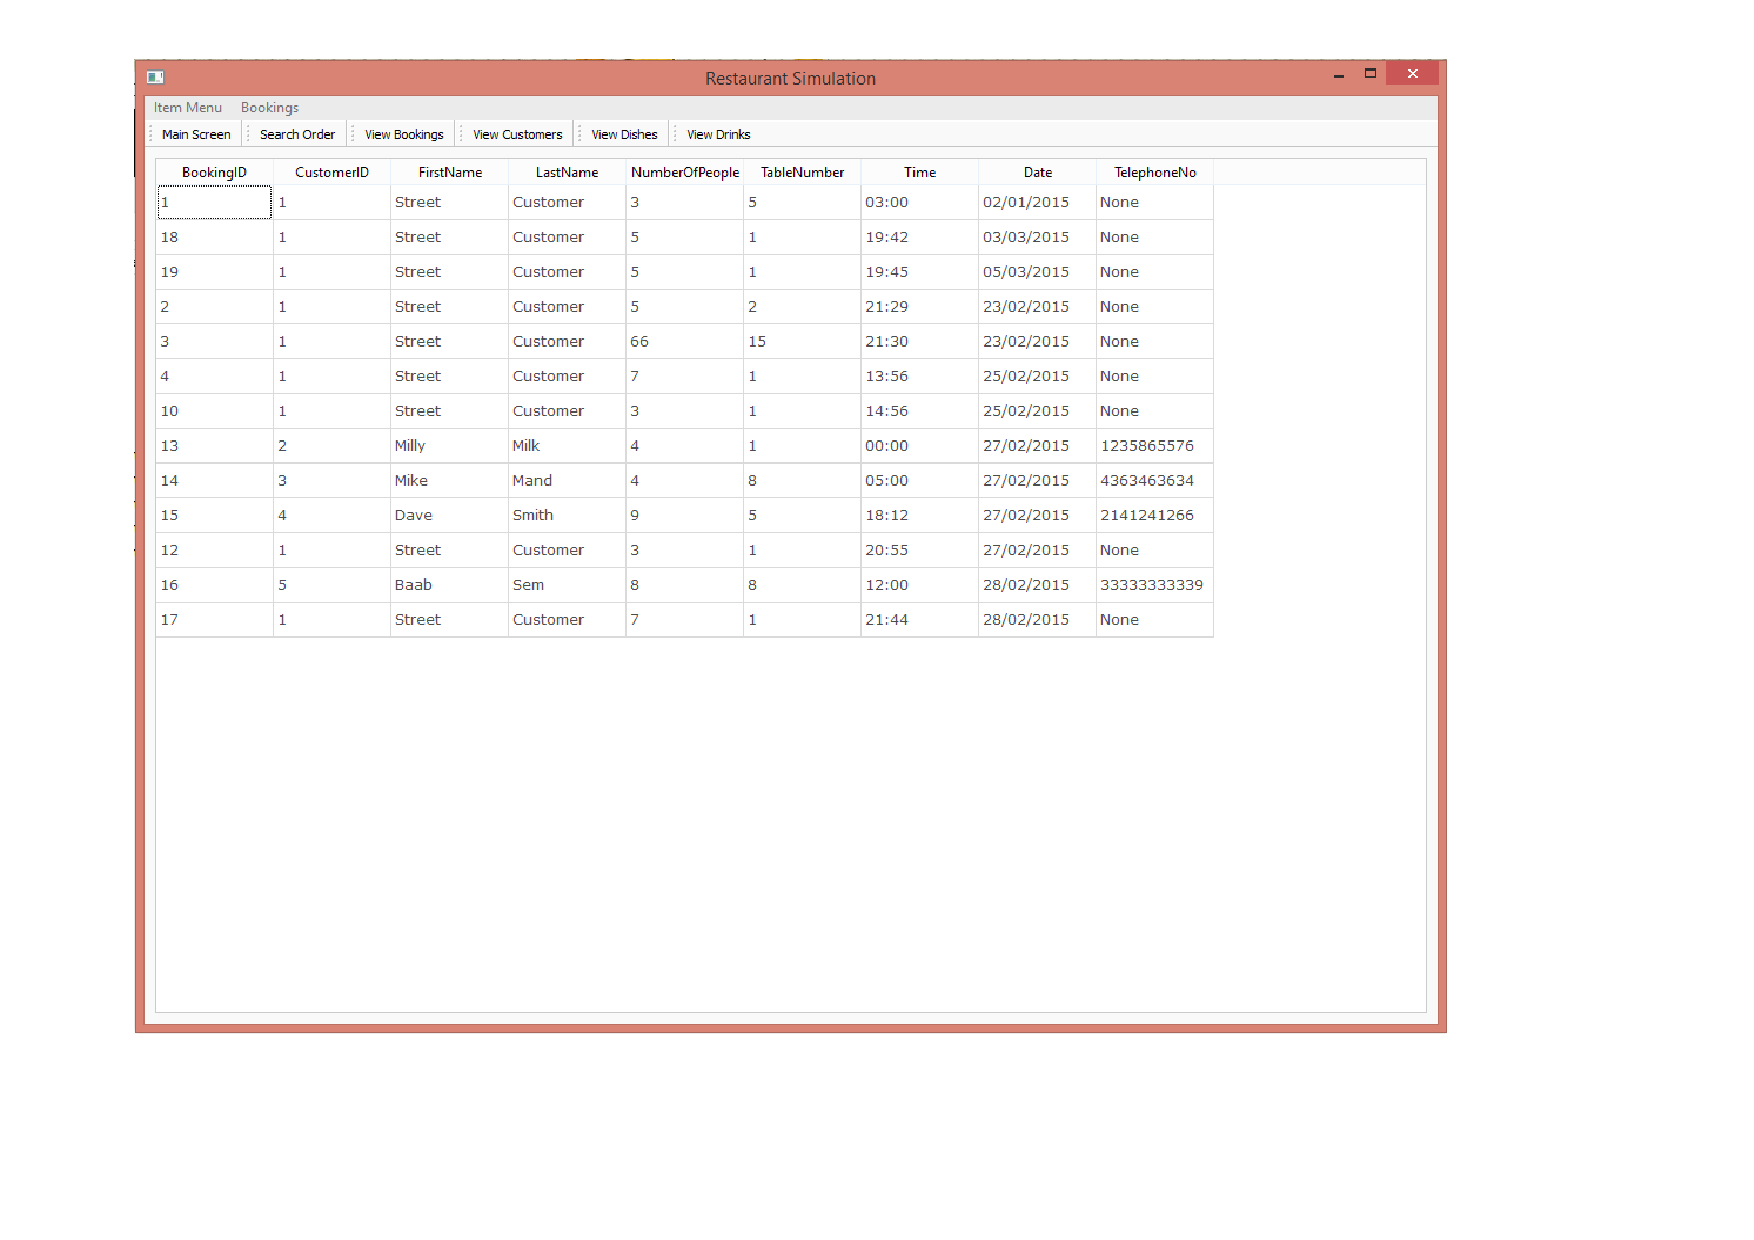
\includegraphics[height = 15cm]{./Maintenance/images/screen18}
    \caption{} \label{fig:screen18}
\end{figure}

\begin{figure}[H]
    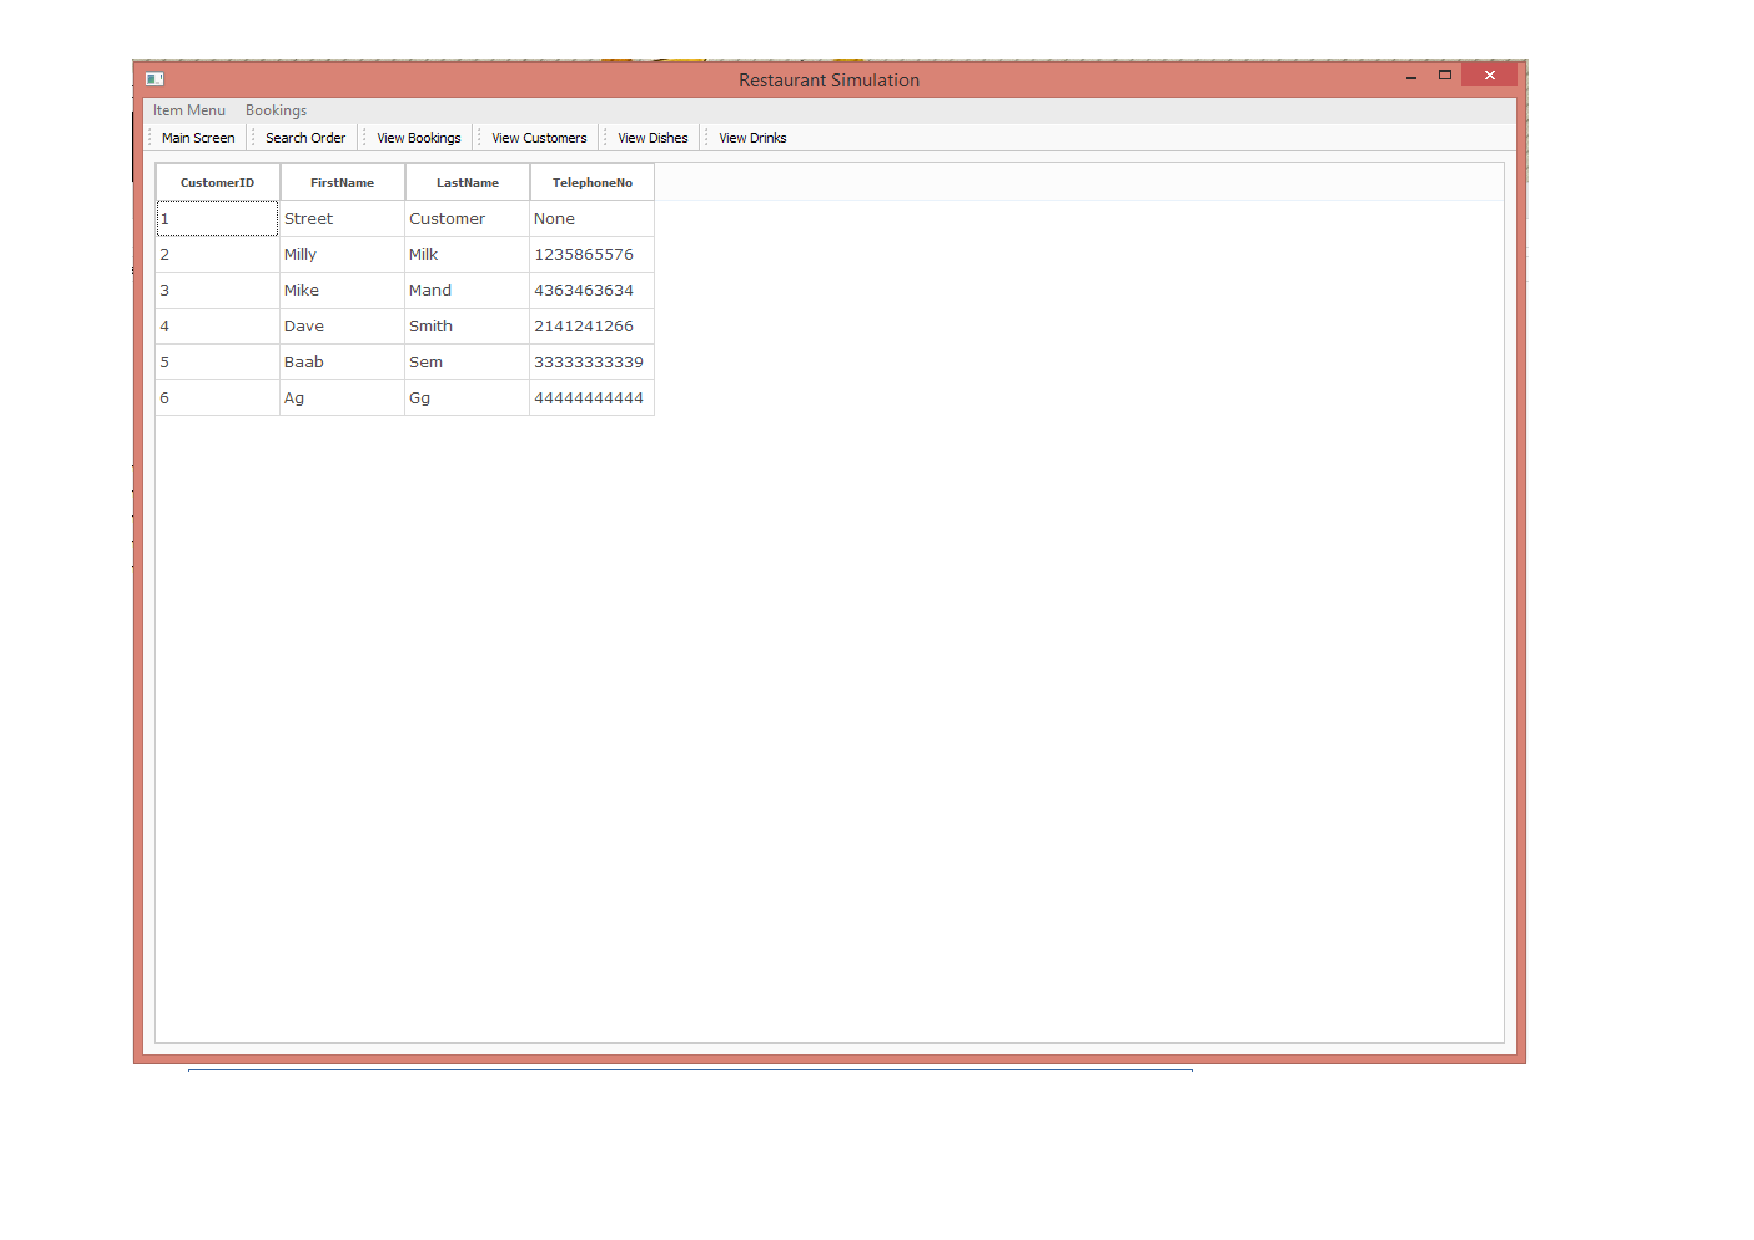
\includegraphics[height = 15cm]{./Maintenance/images/screen19}
    \caption{} \label{fig:screen19}
\end{figure}

\begin{figure}[H]
    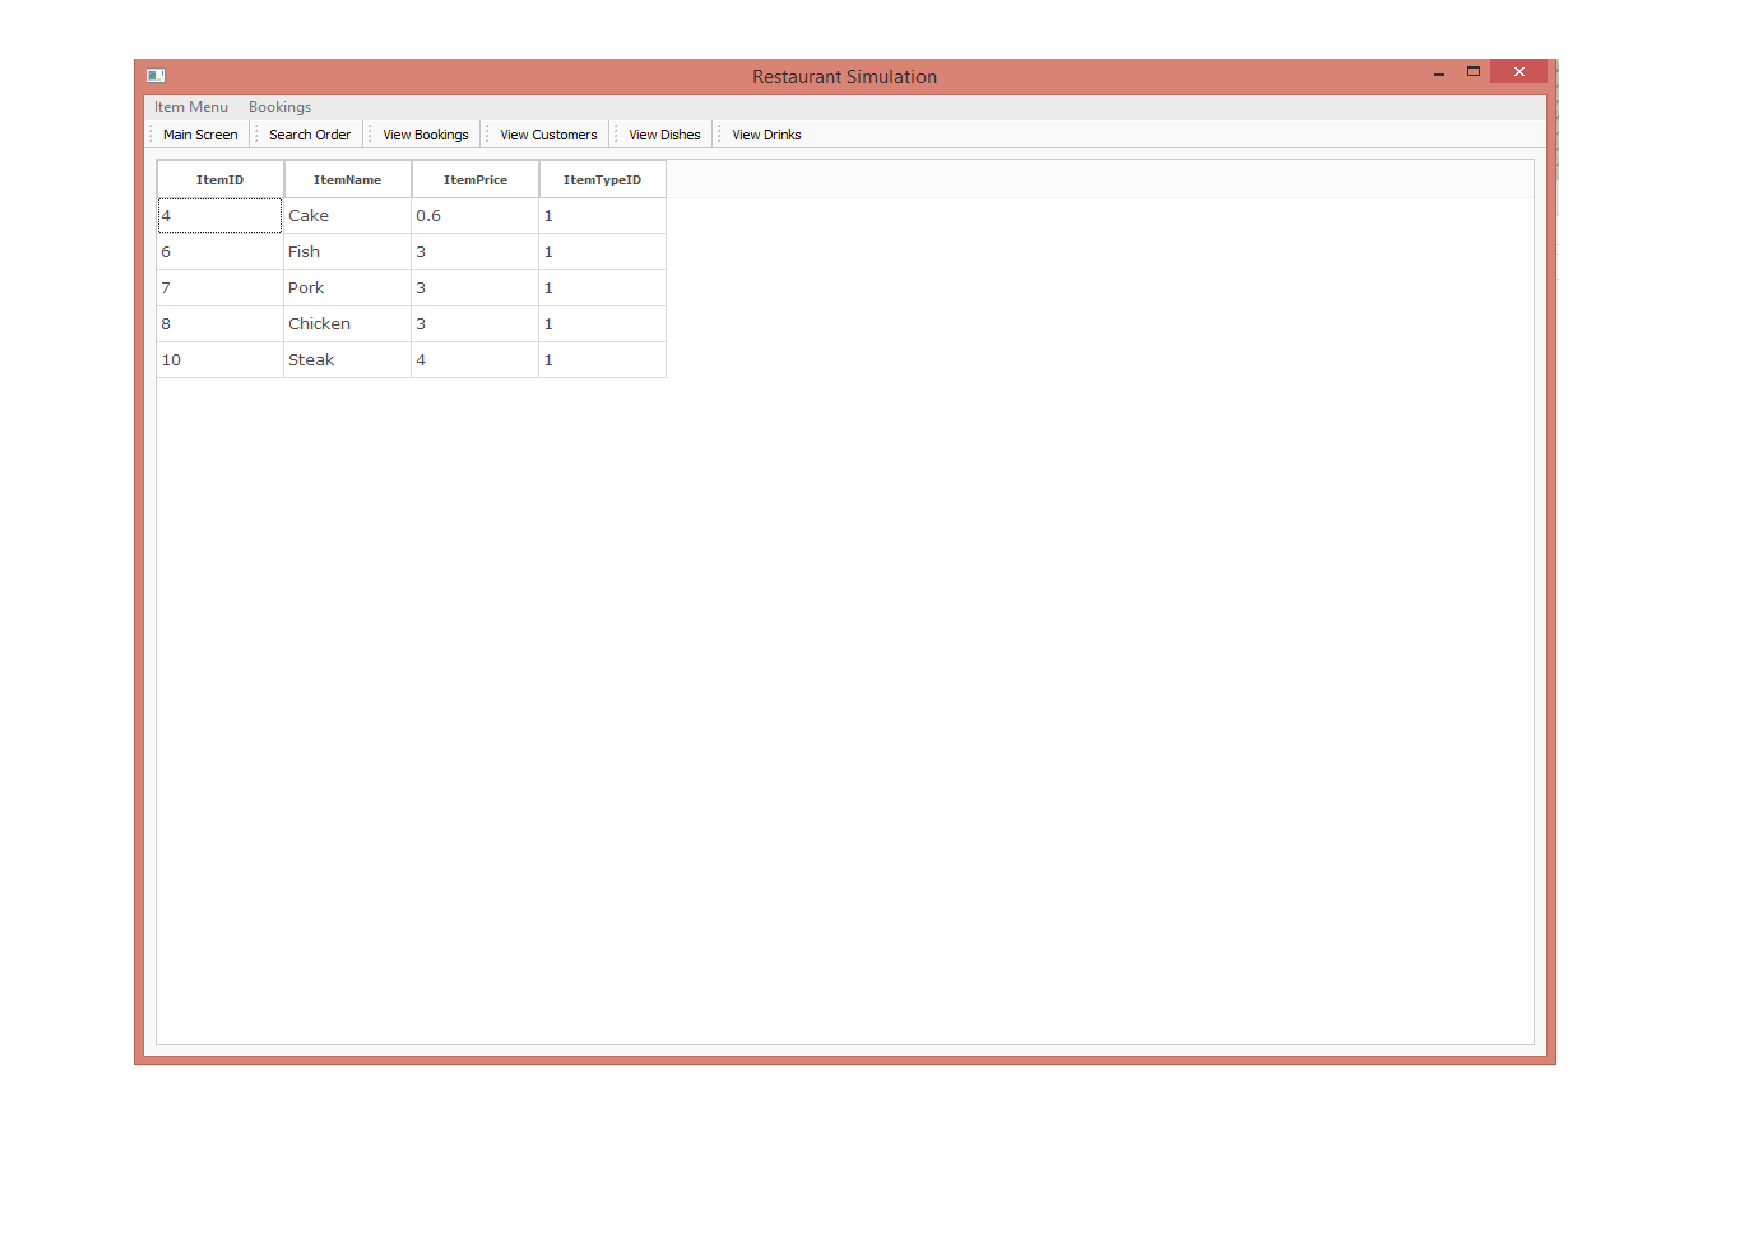
\includegraphics[height = 15cm]{./Maintenance/images/screen20}
    \caption{} \label{fig:screen20}
\end{figure}

\begin{figure}[H]
    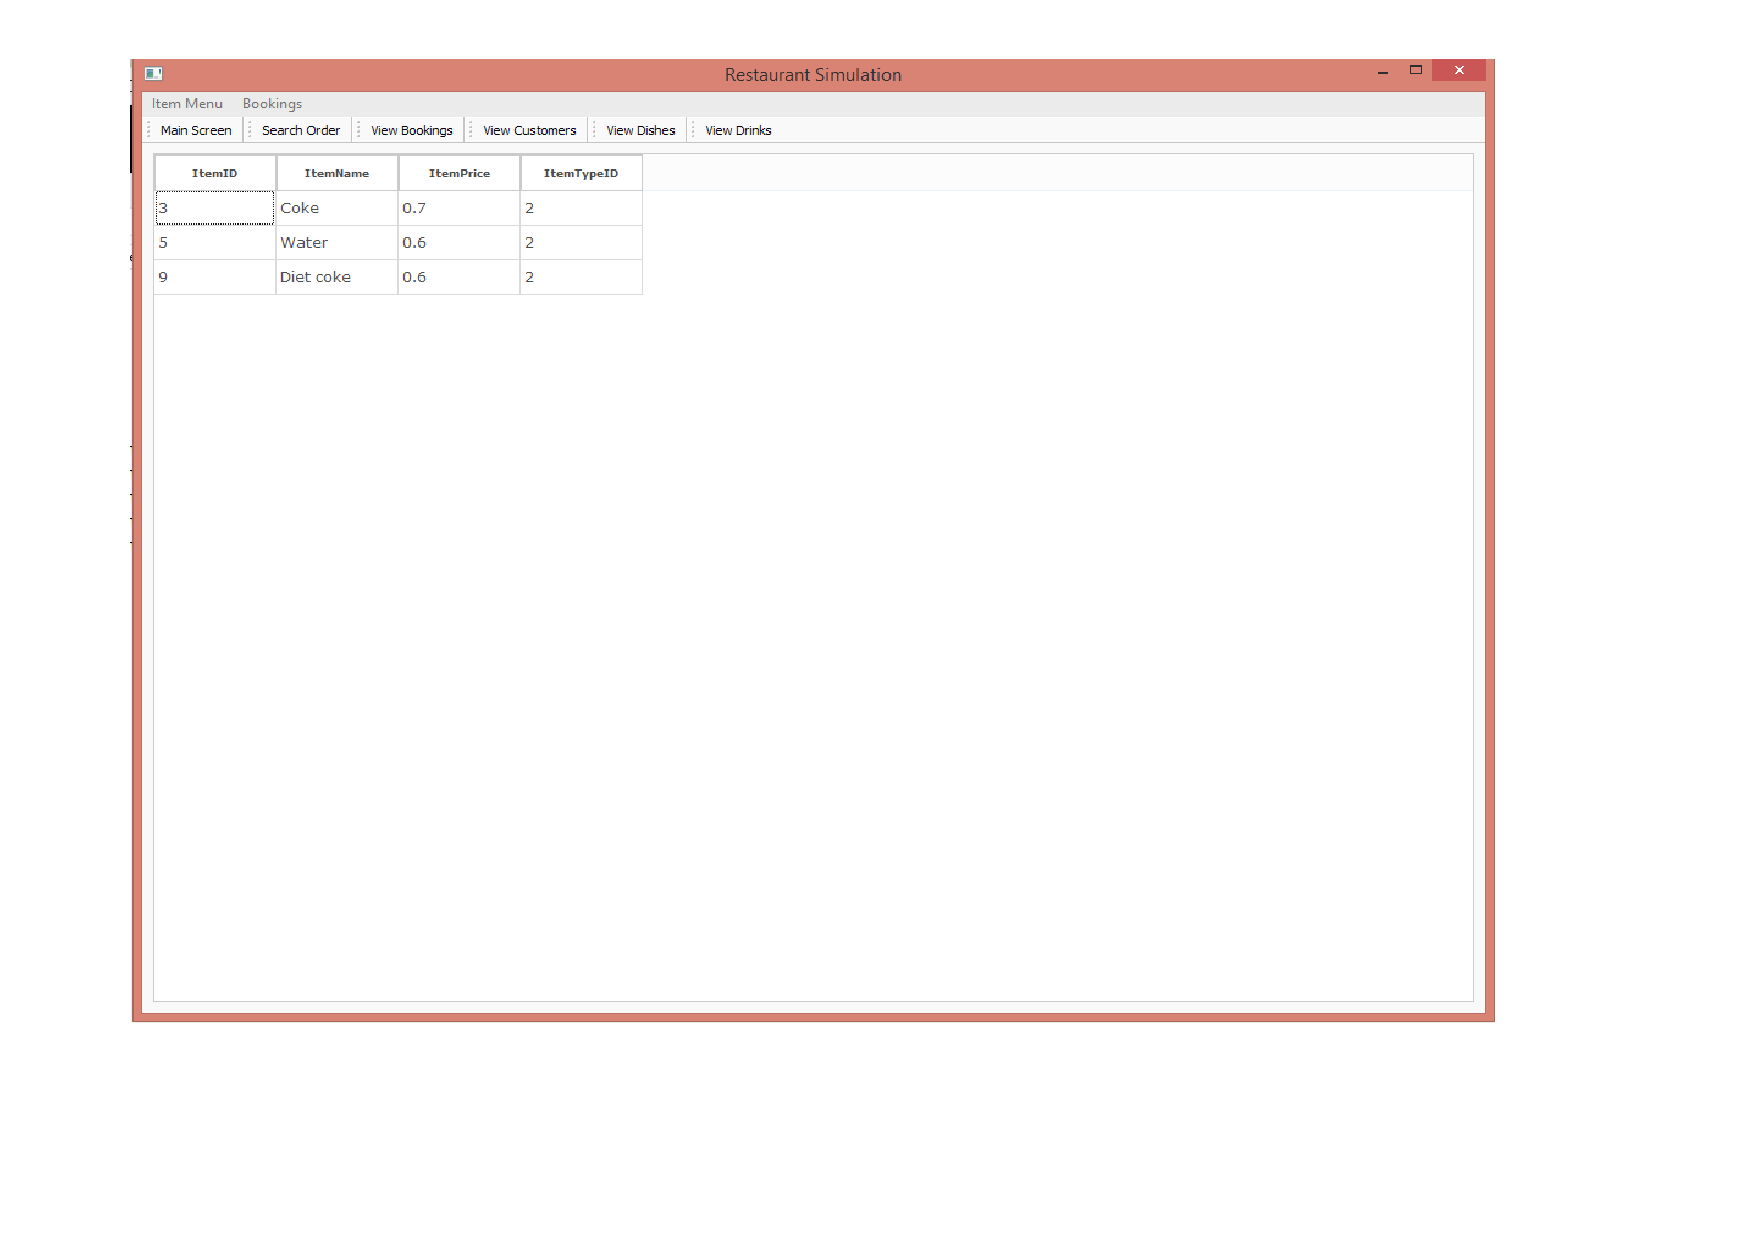
\includegraphics[height = 15cm]{./Maintenance/images/screen21}
    \caption{} \label{fig:screen21}
\end{figure}
\end{landscape}

\subsection{ER Diagram}
\begin{figure}[H]
    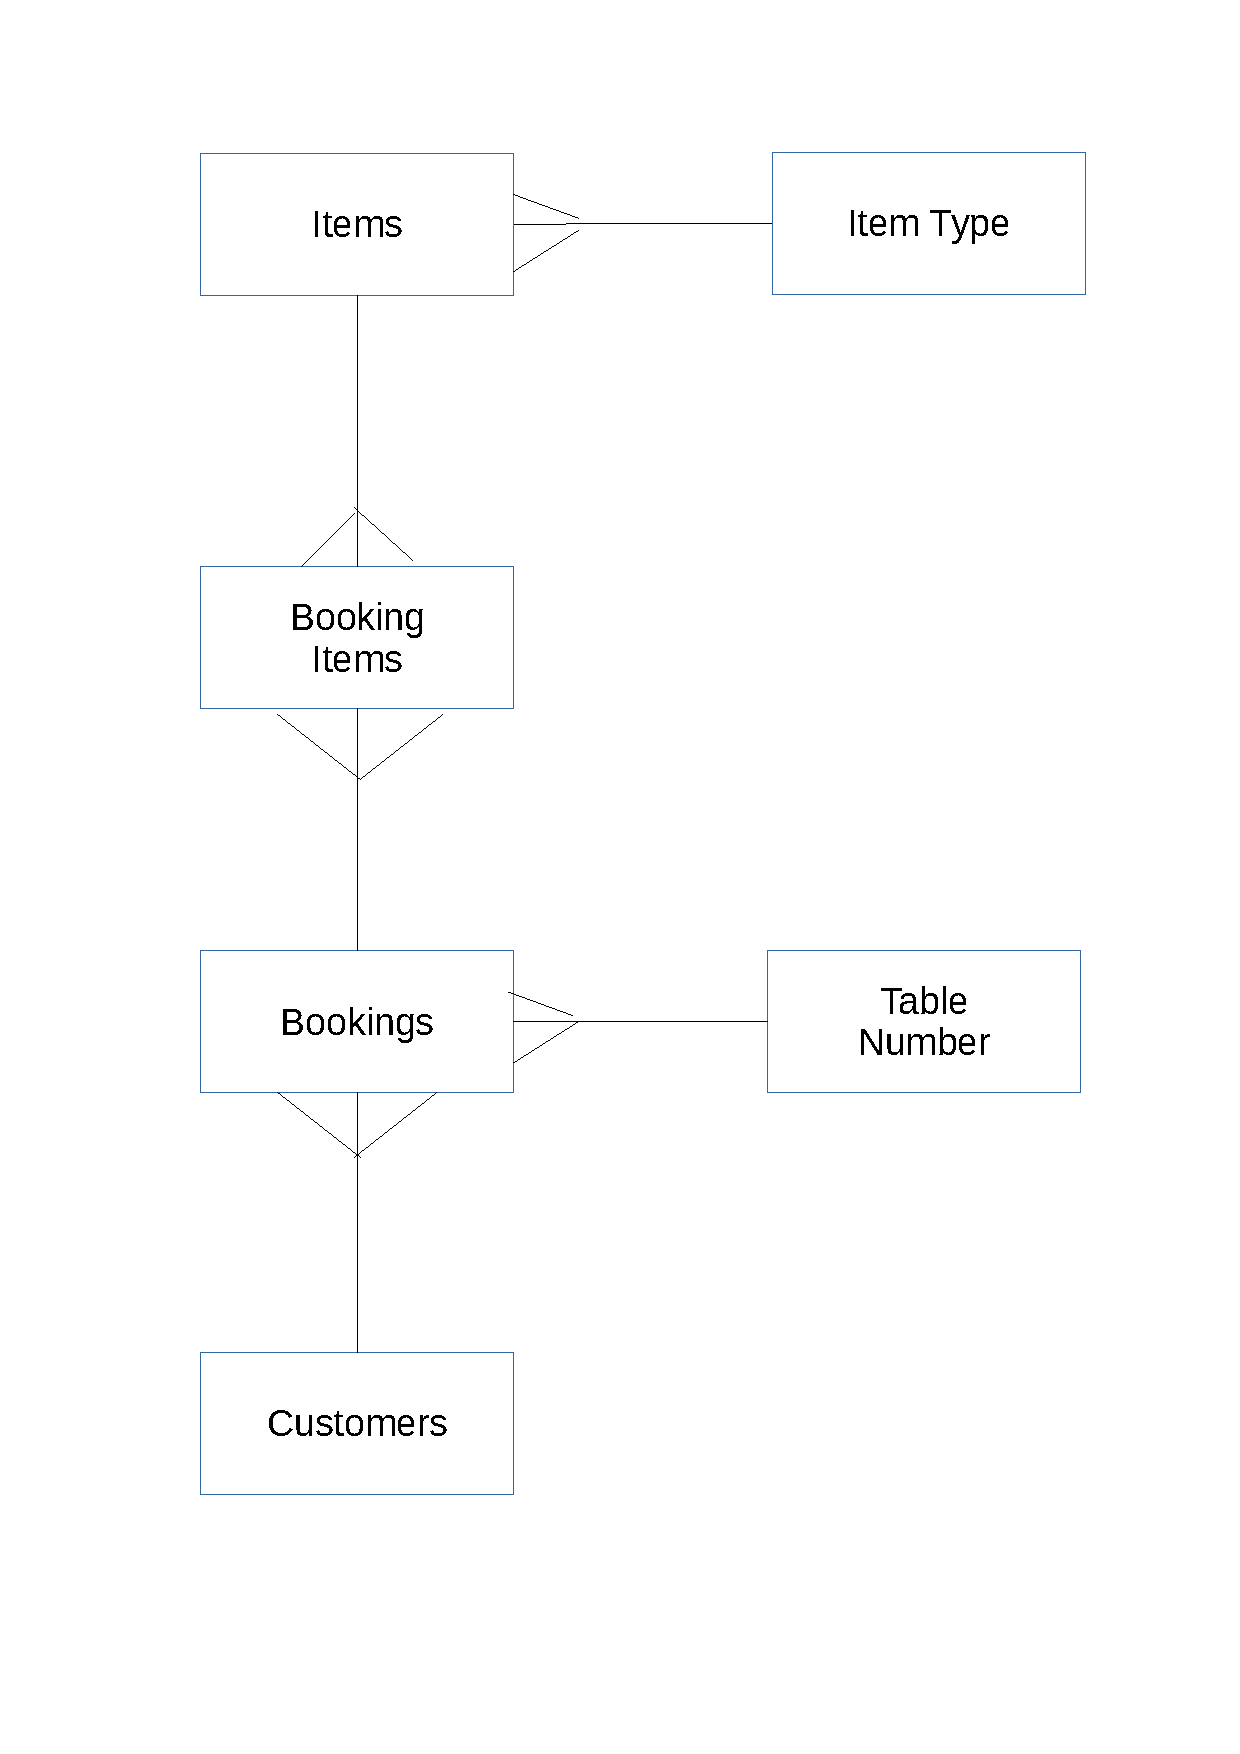
\includegraphics[height = 15cm]{./Maintenance/images/erDiagram}
    \caption{ER Diagram of finished database} \label{fig:erDiagram}
\end{figure}

\subsection{Database Table Views}

\begin{figure}[H]
    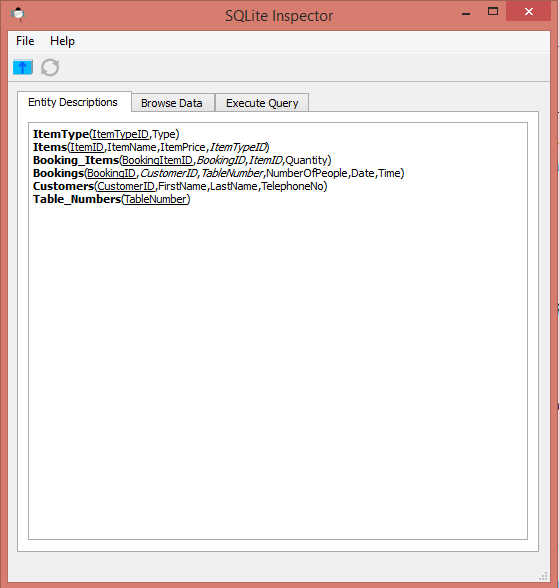
\includegraphics[height = 15cm]{./Maintenance/images/entities}
    \caption{ER Diagram of finished database} \label{fig:entities}
\end{figure}

\begin{figure}[H]
    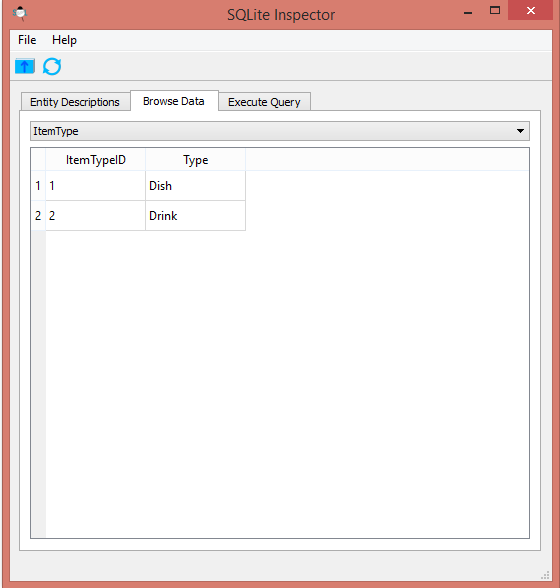
\includegraphics[height = 15cm]{./Maintenance/images/itemtype}
    \caption{Item Type entity} \label{fig:itemtype}
\end{figure}

\begin{figure}[H]
    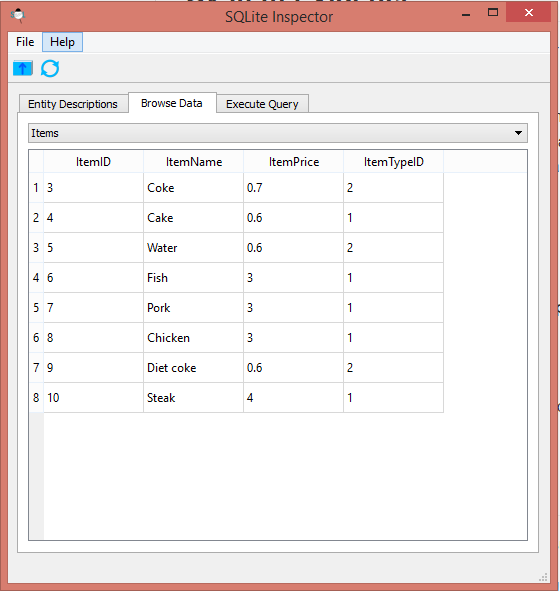
\includegraphics[height = 15cm]{./Maintenance/images/items}
    \caption{Items entity} \label{fig:items}
\end{figure}

\begin{figure}[H]
    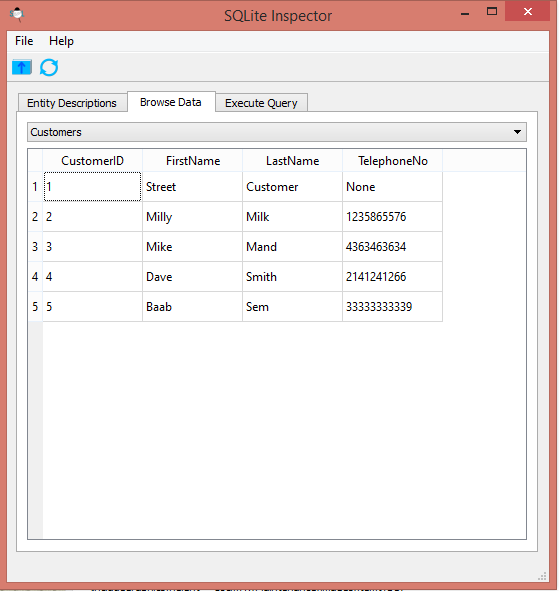
\includegraphics[height = 15cm]{./Maintenance/images/customers}
    \caption{Customers entity} \label{fig:customers}
\end{figure}

\begin{figure}[H]
    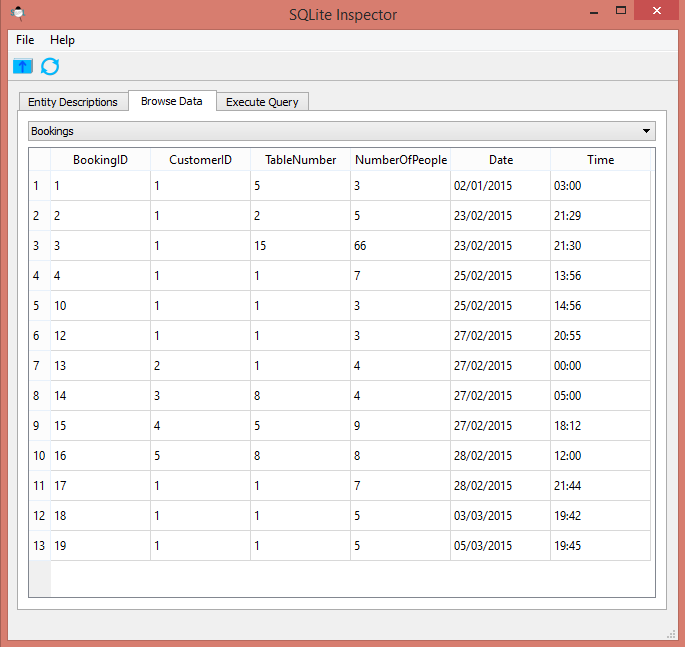
\includegraphics[height = 15cm]{./Maintenance/images/bookings}
    \caption{Bookings entity} \label{fig:bookings}
\end{figure}

\begin{figure}[H]
    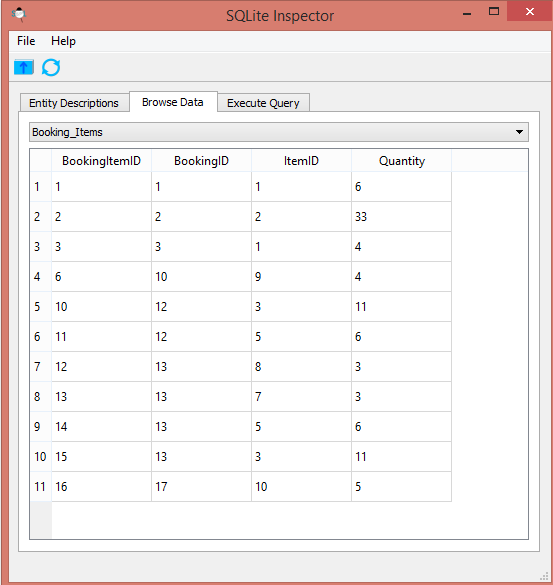
\includegraphics[height = 15cm]{./Maintenance/images/bookingitems}
    \caption{Booking Items entity} \label{fig:bookingitems}
\end{figure}

\newpage
\subsection{Database SQL}

\begin{sql}
CREATE TABLE ItemType(
    ItemTypeID integer,
    Type text,
    Primary Key(ItemTypeID));
\end{sql}

\begin{sql}
CREATE TABLE Items(
             ItemID integer,
             ItemName text,
             ItemPrice real,
             ItemTypeID integer,
             Primary Key(ItemID),
             Foreign Key(ItemTypeID) references ItemType(ItemTypeID));
\end{sql}

\begin{sql}
CREATE TABLE Booking_Items(
    BookingItemID integer,
    BookingID integer,
    ItemID  integer,
    Quantity integer,
    Primary Key(BookingItemID)
    Foreign Key (BookingID) references Bookings(BookingIDID) on delete cascade,
    Foreign Key(ItemID) references Items(ItemID));
\end{sql}

\begin{sql}
CREATE TABLE Bookings(
	BookingID integer,
             CustomerID integer,
             TableNumber integer,
             NumberOfPeople integer,
             Date text,
             Time text,
             Primary Key(BookingID),
             Foreign Key(CustomerID) references Customers(CustomerID),
             Foreign Key(TableNumber) references Table_Numbers(TableNumber)));
\end{sql}

\begin{sql}
CREATE TABLE Table_Numbers(
    TableNumber integer,
    Primary Key(TableNumber));
\end{sql}

\begin{sql}
CREATE TABLE Customers(
             CustomerID integer,
             FirstName text,
             LastName text,
             TelephoneNo integer,
             Primary key(CustomerID));
\end{sql}

\subsection{SQL Queries}

\subsubsection{Used to create customer records}
\begin{sql}
insert into Customers (FirstName,LastName,TelephoneNo) values (?,?,?)
\end{sql}

\subsubsection{Used to create the item types}
\begin{sql}
insert into ItemType (Type) values (?)
\end{sql}

\subsubsection{Used to insert the table numbers}
\begin{sql}
insert into Table_Numbers (TableNumber) values (?)
\end{sql}

\subsubsection{Used to get a customer id}
\begin{sql}
select CustomerID from Customers where TelephoneNo=? and FirstName=? and LastName=?
\end{sql}

\subsubsection{Used to create a booking}
\begin{sql}
insert into Bookings(CustomerID, TableNumber, NumberOfPeople, Date, Time) values (?,?,?,?,?)
\end{sql}

\subsubsection{Used to insert an item to the menu}
\begin{sql}
insert into Items(ItemName,ItemPrice,ItemTypeID) values (?,?,?)
\end{sql}

\subsubsection{Used to get quantity of an ordered item}
\begin{sql}
select Quantity from Booking_Items where ItemID=? and BookingID = ?
\end{sql}

\subsubsection{Used to update the quantity of an ordered item}
\begin{sql}
update Booking_Items set Quantity=? where ItemID=?
\end{sql}

\subsubsection{Used to add an item to an order}
\begin{sql}
insert into Booking_Items(BookingID,ItemID,Quantity) values (?,?,?)
\end{sql}


\begin{sql}
SELECT
Items.ItemName
FROM Items
 INNER JOIN Booking_Items
ON Booking_Items.ItemID = Items.ItemID
WHERE Booking_Items.BookingID = ?
\end{sql}
This query fetches all the item names that have been ordered, given the  booking id.  \\ \\

\begin{sql}
SELECT
 Items.ItemName
 FROM Items
INNER JOIN Booking_Items
ON Booking_Items.ItemID = Items.ItemID
 WHERE Booking_Items.BookingID = ?
 AND Items.ItemID = ?
\end{sql}
This query fetches the item name of an ordered item, given the booking id and item id. \\ \\

\begin{sql}
SELECT
 Customers.FirstName,
 Customers.LastName,
 Bookings.NumberOfPeople,
 Bookings.Time
 FROM Customers
INNER JOIN Bookings
ON Customers.CustomerID = Bookings.CustomerID
WHERE Bookings.Date = '{0}'
AND Bookings.TableNumber = {1}
.format(self.systemdate,TableNumber)
\end{sql}
This query fetches all the bookings that matches the system date and the relevant table number with the customer's first name, last name, number of people and booking time. \\ \\

\subsubsection{Used to get booking details of a customer}

\begin{sql}
select * from Bookings where CustomerID = {0} and TableNumber = {1} and NumberOfPeople = {2} and Date = '{3}' and Time = '{4}' .format(CustomerID,TableNumber,NumberOfPeople,Date,Time))
\end{sql}

\subsection{Used to get booking details for the selected table and the date that matches the computer system}
\begin{sql}
select * from Bookings where CustomerID = {0} and TableNumber = {1} and Date = '{2}'.format(CustomerID,self.tableNumber,TodaysDate)
\end{sql}


\subsubsection{Used to get the customer ID of a booking on the selected table and the date that matches the computer system}
\begin{sql}
select CustomerID from Bookings where TableNumber = {0} and Date = '{1}'.format(TableNumber,TodaysDate)
\end{sql}

\subsubsection{Used to get the last name of a customer}

\begin{sql}
select LastName from Customers where CustomerID = {0}.format(customer))
\end{sql}

\subsubsection{Used to delete a booking}
\begin{sql}
delete from Bookings where BookingID = {0}.format(booking)
\end{sql}

\subsubsection{Used to delete an item off the item menu given the name of the item}
\begin{sql}
delete from Items where ItemName = ?
\end{sql}

\subsubsection{Used to delete an item off the item menu given the ID of the item}
\begin{sql}
delete from Items where ItemID = {0}.format(itemID)
\end{sql}

\subsubsection{Used to delete ordered items off the selected booking}
\begin{sql}
delete from Booking_Items where BookingID = ? and ItemID = ? 
\end{sql}

\begin{sql}
SELECT
 Customers.FirstName,
Customers.LastName,
 Bookings.NumberOfPeople,
 Bookings.TableNumber,
 Bookings.Time
FROM Customers
 INNER JOIN Bookings
 ON Customers.CustomerID = Bookings.CustomerID
 WHERE Bookings.Date = '{0}'
 ORDER BY Bookings.Time
.format(TodaysDate)
\end{sql}
This query fetches all the bookings that matches the booking date with the system'sdate with its details including customer details. \\ \\

\begin{sql}
SELECT
 Bookings.BookingID,
 Customers.CustomerID,
Customers.FirstName,
Customers.LastName,
Bookings.NumberOfPeople,
 Bookings.TableNumber,
 Bookings.Time,
Bookings.Date,
Customers.TelephoneNo
 FROM Customers
 INNER JOIN Bookings
 ON Customers.CustomerID = Bookings.CustomerID
 ORDER BY Bookings.Date,Bookings.Time
\end{sql}
This query gets all the records from the bookings entity as well as the customer records that matches with the bookings. \\ \\

\begin{sql}
SELECT
Booking_Items.Quantity,
 Items.ItemName,
 Items.ItemPrice
 FROM Items
 INNER JOIN Booking_Items
ON Booking_Items.ItemID = Items.ItemID
 WHERE Booking_Items.BookingID = {0}
AND Items.ItemTypeID = 2
\end{sql}
This query fetches all the ordered drinks , given the booking id. \\ \\

\begin{sql}
SELECT
 Booking_Items.Quantity,
 Items.ItemName,
 Items.ItemPrice
 FROM Items
 INNER JOIN Booking_Items
ON Booking_Items.ItemID = Items.ItemID
 WHERE Booking_Items.BookingID = {0}
 AND Items.ItemTypeID = 1
\end{sql}
This query fetches all the ordered dishes, given the booking id. \\ \\

\begin{sql}
SELECT
Items.ItemPrice
 FROM Items
 INNER JOIN Booking_Items
 ON Booking_Items.ItemID = Items.ItemID
WHERE Booking_Items.BookingID = ?
\end{sql}
This query fetches the prices of each ordered item \\ \\


\begin{sql}
SELECT
 Booking_Items.Quantity
 FROM Items
 INNER JOIN Booking_Items
 ON Booking_Items.ItemID = Items.ItemID
 WHERE Booking_Items.BookingID = ? 
\end{sql}
This query fetches the quantiity of each ordered item \\ \\

\begin{sql}
SELECT
 Booking_Items.Quantity,
 Items.ItemName,
 Items.ItemPrice
 FROM Items
 INNER JOIN Booking_Items
 ON Booking_Items.ItemID = Items.ItemID
 WHERE Booking_Items.BookingID = {0}
\end{sql}
This query fetches all the ordered items with its information such as quantity, name and price \\ \\

\subsubsection{Used to update the booking date, given the ID}
\begin{sql}
update Bookings set Date=? where BookingID=?
\end{sql}

\subsubsection{Used to update the booking time, given the ID}
\begin{sql}
update Bookings set Time=? where BookingID=?
\end{sql}

\subsubsection{Used to update the number of people expected for the selected booking, given the ID}
\begin{sql}
update Bookings set NumberOfPeople=? where BookingID=?
\end{sql}

\subsubsection{Used to update the table number of the booking, given the ID}
\begin{sql}
update Bookings set TableNumber=? where BookingID=?
\end{sql}

\subsubsection{Used to update the price of an item}
\begin{sql}
update Items set ItemPrice=? where ItemID=?
\end{sql}

\section{Testing}

\subsection{Summary of Results}
After completing the series of tests, i believe that my application is reliable and robust as the majority of the results were expected and the application did not crash whilst carrying out these tests ( See page 87 for testing). I used diferrent types of test data such as normal, erroneous and boundery whenever possible to test if my application would crash or give errors - The errors were handled using exceptions and I didn't experience any crashes which is why I believed my application is robust.However, there was a weakness to my testing as I did not test all radio buttons on the main screen.


\subsection{Known Issues}

\subsubsection{Test 4.03 - Manage order total price}
There was a problem with the manage order box where the Total Price was suppose to be displayed. The problem was that it was suppose to display the total price after adding an item to the order or deleting an item off the order which it didn't (The widget didn't refresh with the new total price). However, I know that the algorithm for the total price is correct because I used the same algorithm for the invoice (which worked as test 4.03.01 was successful). At this current time, I am not sure how to fix it in terms of coding but I do know that the problem is that the line edit doesn't refresh with the new value.


\section{Code Explanations}

\subsection{Difficult Sections}

\newpage
\subsection{Select function (section 4.10.4)}
\pythonfile[firstline=148, lastline=163]{./Implementation/GUI/assign_table_customer.py}

Above is a function thats connected to the Select button as shown by Figure \ref{fig:screen9} on page \pageref{fig:screen9}. This function is used to return the booking details of the selected customer from the combo box beside it. Below is a table explaining code.


\begin{center}
\begin{tabular}{|p{5cm}|p{7.5cm}|}
\hline
\textbf{Line Number} & \textbf{Explanation} \\ \hline
2 & Assigns the system's date to TodaysDate \\ \hline
3 & Assigns the selected index(customer) of the combo box to customerCurrentIndex \\ \hline
5 & Gets the customerID of the selected customer using the list self.CustomerList and assigns it to CustomerID \\ \hline
10 & SQL statement to get the booking details of the selected customer  \\ \hline
11 & The booking details is assigned to self.bookingDetails \\ \hline
14 & self.close() closes the assign customer to table box \\ \hline

\end{tabular}
\end{center}
\newpage
\subsection{Creating the combo box (section 4.10.4)}
\pythonfile[firstline=165, lastline=189]{./Implementation/GUI/assign_table_customer.py}

Above is a function that creates the combo box and populates it with customer last names of bookings that match the system date. The combo box is shown by Figure \ref{fig:screen9} on page \pageref{fig:screen9} but it is not populated in that image. Below is a table explaining the code

\begin{center}
\begin{tabular}{|p{5cm}|p{7.5cm}|}
\hline
\textbf{Line Number} & \textbf{Explanation} \\ \hline
4 & Assigns the system's date to TodaysDate \\ \hline
10 & SQL statement to get all the customer IDs that have a booking on table (tablenumber) and matches the system date.  \\ \hline
11-12 & A FOR loop to append the self.CustomerList with the customer ids fetched from line 10 \\ \hline
15-18 & SQL statement to get all the last names of the customer ids in the self.CustomerList array \\ \hline
20 & Appends the CustomerLastName list with the last names from lines 15-18 \\ \hline
23-25 & Creates the combo box and uses a FOR loop to populate the combobox with the last names \\ \hline


\end{tabular}
\end{center}

\newpage
\subsection{Self-created Algorithms}
\pythonfile[firstline=226, lastline=238]{./Implementation/GUI/main_window.py}
The above algorithm is used to tell the program if the table is occupied or not. Below is a table explaining the algorithm in more depth.

\begin{center}
\begin{tabular}{|p{5cm}|p{7.5cm}|}
\hline
\textbf{Line Number} & \textbf{Explanation} \\ \hline
1 & If the selected table number radio button is 1 then the algorithm will proceed \\ \hline
2 & If the table is not occupied then lines 3-8 will proceed \\ \hline
3 & The assign customer box will pop up and user would have to create a booking from there or select a booking ( Figure \ref{fig:screen9} on page \pageref{fig:screen9}) \\ \hline
4 & The booking details is returned if the user has created or selected a booking \\ \hline
5 & The assign customer box will close and the manage order box will pop up  (Figure \ref{fig:screen10} on page \pageref{fig:screen10}) \\ \hline
6 & The table is now occupied \\ \hline
7-8 & If the user presses the Finish button on the manage order box without closing it then the table will be set as unoccupied \\ \hline
9 & This part of the algorithm will only proceed if the user closes the box without pressing Finish \\ \hline
10 & The booking details is returned to pass it to the manage order box \\ \hline
11& Manage order box pops up \\ \hline
12-13 & If the user presses the Finish button then the table will be set as unoccupied \\ \hline
 
\end{tabular}
\end{center}

\newpage
\pythonfile[firstline=96, lastline=130]{./Implementation/GUI/add_item_to_order.py}
The algorithm above is used to check if an item that is about to be added has already been ordered, if it has then the quantity will increase(quantity increase is not part of this algorithm). I created a list (line 3) which was used to populate it (line 14-16)with all ordered items from the relevent booking. I then got the item name that was going to be added to the order (lines 21-28) and checked if the item was in the list that was populated with the ordered items (lines 32-33).

\newpage

\pythonfile[firstline=123, lastline=141]{./Implementation/GUI/delete_item_off_order.py}
The algorithm above will be used when the user wants to delete an item off an order. It is used to find out if the quantity of the item that wants to be deleted has a quantity of one or not. Lines 4-11 gets the quantity of the ordered item that the user wants to delete and if the quantity is equal to 1 then OneQuantity will be set to True if not then the returned OneQuantity will be False. 
\section{Settings}

My client's computer system settings will not need any changes to run the application as I have made the application an executable however, if anyone wanted to alter the application then Python and PyQt4 would be needed.

\section{Acknowledgements}

I used http://doc.qt.digia.com/4.6/stylesheet-reference.html to help me with the style sheets for my application. I did not copy any coding but I did use the website's examples to help me understand what was needed to create the cascade style sheet. For example there was an example \\
" The background color used for the widget. \\
Examples: \\ \\
 QLabel { background-color: yellow } \\
 QLineEdit { background-color: rgb(255, 0, 0) }"
\\ \\
In addition, I used http://pyqt.sourceforge.net/Docs/PyQt4/qtsql.html to help me display sql tables. The example that helped me the most was \\
"QSqlTableModel offers a read-write model that works on a single SQL table at a time. \\
\\
Example:
\\
        QSqlTableModel model; \\
        model.setTable("employee"); \\
        model.setFilter("salary > 50000"); \\
        model.setSort(2, Qt.DescendingOrder); \\
        model.select(); \\
"

\section{Code Listing}
\begin{landscape}
%include as many subsections as you have modules
\subsection{add\_booking.py}
%the code below can be uncommented and used to get a code section from a particular file
\pythonfile[firstline=1]{./Implementation/GUI/add_booking.py}

\subsection{add\_item\_to\_menu.py}
\pythonfile[firstline=1]{./Implementation/GUI/add_item_to_menu.py}

\newpage
\subsection{add\_item\_to\_order.py}
\pythonfile[firstline=1]{./Implementation/GUI/add_item_to_order.py}

\newpage
\subsection{assign\_table\_customer.py}
\pythonfile[firstline=1]{./Implementation/GUI/assign_table_customer.py}

\newpage
\subsection{cascade\_style\_sheet.py}
\pythonfile[firstline=1]{./Implementation/GUI/cascade_style_sheet.py}

\newpage
\subsection{delete\_booking.py}
\pythonfile[firstline=1]{./Implementation/GUI/delete_booking.py}

\newpage
\subsection{delete\_item\_off\_menu.py}
\pythonfile[firstline=1]{./Implementation/GUI/delete_item_off_menu.py}

\newpage
\subsection{delete\_item\_off\_order.py}
\pythonfile[firstline=1]{./Implementation/GUI/delete_item_off_order.py}

\newpage
\subsection{main\_window.py}
\pythonfile[firstline=1]{./Implementation/GUI/main_window.py}

\newpage
\subsection{manage\_booking.py}
\pythonfile[firstline=1]{./Implementation/GUI/manage_booking.py}

\newpage
\subsection{manage\_order.py}
\pythonfile[firstline=1]{./Implementation/GUI/manage_order.py}

\newpage
\subsection{new\_create\_tables\_cli.py}
\pythonfile[firstline=1]{./Implementation/GUI/new_create_tables_cli.py}

\newpage
\subsection{print\_invoice.py}
\pythonfile[firstline=1]{./Implementation/GUI/print_invoice.py}

\newpage
\subsection{radio\_button\_widget\_class.py}
\pythonfile[firstline=1]{./Implementation/GUI/radio_button_widget_class.py}

\newpage
\subsection{search\_order.py}
\pythonfile[firstline=1]{./Implementation/GUI/search_order.py}

\newpage
\subsection{table\_display.py}
\pythonfile[firstline=1]{./Implementation/GUI/table_display.py}

\newpage
\subsection{update\_booking.py}
\pythonfile[firstline=1]{./Implementation/GUI/update_booking.py}

\newpage
\subsection{update\_item\_price.py}
\pythonfile[firstline=1]{./Implementation/GUI/update_item_price.py}


\end{landscape}
